\documentclass[english]{article}[12pt]
\usepackage{graphicx}
\usepackage[T1]{fontenc}
\usepackage[latin9]{inputenc}
\usepackage{amstext}
\usepackage{amsmath}
\usepackage{amsfonts}
\usepackage{amssymb}
\usepackage{babel}
\usepackage{courier}
\usepackage[margin=1in]{geometry}
\usepackage{graphicx}
\usepackage{caption}
\usepackage{subfigure}

\begin{document}

\title{Final Documentation: \\Matrix Product States for Probability Dynamics}


\author{Peter Gjeltema (gjeltema@princeton.edu)
	   \\ Peiqi Wang (peiqiw@princeton.edu)
	    \\ Jun Xiong (xiong@princeton.edu) 
	    \\ Bin Xu (binx@princeton.edu) 
	    \\ Liangsheng Zhang(liangshe@princeton.edu)}
	    
\date{\today}

\maketitle

\section{Introduction}

The matrix product state (MPS) is a novel numerical algorithm that is
widely used in quantum many-body physics. For a problem of quantum
spin chains, the states live in a Hilbert space expanded by the states
of each spin (referred to as ``orbitals'' hereafter), and the dimension
of that Hilbert space is $m^{N}$ for a chain of length $N$ where each orbital has $m$ choices. 
The dimension of the state space
grows exponentially with $N$, making it extremely hard to simulate
a system consisting of a few dozen sites. 

In 1995, White \cite{white} proposed
the density matrix renormalization group (DMRG), which proves to be an extremely efficient algorithm for one dimensional systems. Researchers of the next decade were aware of the ubiquitous relation between entanglement and dimensionality allowing the state to be approximated as the product of matrices \cite{schollwock}. Some recent developments include extension of the algorithm to higher dimensions\cite{cirac} and to critical systems\cite{vidal}.

This inter-departmental collaborative work applies this algorithm to other interesting problems. The algorithm's inherent probabilistic nature motivates its application to other difficult problems in probability theory and stochastic processes. An especially interesting example is the Markov process consisting of many degrees of freedom, which also forms an exponentially growing state space. 

We have developed  a generic MPS solver and compare results from some simple applications with that of exact transition matrix solutions. We start with a simple model of the dynamics of human relations (``Angry Boys" model), and move on to include other more sophisticated models. Due to the time limitation, this project focuses on one dimensional models for which the algorithm is well-established in physics. Higher dimensionality or highly correlated relationships offering the most realistic relevance will be left to future work.

\section{Background}

\subsection{The difficult many body problem}

When we have a state as a vector in the Hilbert space, it is expressed
as

\[
|\psi\rangle=\sum_{\{\sigma_{i}\}}A_{\{\sigma_{i}\}}|\sigma_{1}\sigma_{2}\sigma_{3}\cdot\cdot\cdot\sigma_{N}\rangle
\]
where $|\sigma_{1}\sigma_{2}\sigma_{3}\cdot\cdot\cdot\sigma_{N}\rangle$
is a product basis of the local Hilbert space on different sites.

Applying a linear time-evolution operator $\hat{O}$ on this state,
the general form of $\hat{O}$ is

\[
\hat{O}=\sum_{\{\sigma\},\{\sigma'\}}|\sigma'_{1}\sigma'_{2}\sigma'_{3}\cdot\cdot\cdot\sigma'_{N}\rangle\langle\sigma_{1}\sigma_{2}\sigma_{3}\cdot\cdot\cdot\sigma_{N}|O_{\{\sigma'\}\{\sigma\}}
\]
where $\langle\sigma_{1}\sigma_{2}\sigma_{3}\cdot\cdot\cdot\sigma_{N}|$ is a vector in the dual Hilbert space and $O_{\{\sigma'\}\{\sigma\}}$ is a complex number that represents the amplitude of transition. The application of this operator on the state is naturally written as
\[
\hat{O}|\psi\rangle=\sum_{\{\sigma\},\{\sigma'\}}|\sigma'_{1}\sigma'_{2}\sigma'_{3}\cdot\cdot\cdot\sigma'_{N}\rangle\langle\sigma_{1}\sigma_{2}\sigma_{3}\cdot\cdot\cdot\sigma_{N}|\ O_{\{\sigma'\}\{\sigma\}}\sum_{\{\sigma''_{i}\}}A_{\{\sigma_{''i}\}}|\sigma''_{1}\sigma''_{2}\sigma''_{3}\cdot\cdot\cdot\sigma''_{N}\rangle
\]
Using the orthonormal condition of basis, it can be simplified to

\[
\hat{O}|\psi\rangle=\sum_{\{\sigma_{i}\}\{\sigma'_{i}\}}A_{\{\sigma_{i}\}}O_{\{\sigma'\}\{\sigma\}}|\sigma'_{1}\sigma'_{2}\sigma'_{3}\cdot\cdot\cdot\sigma'_{N}\rangle
\]


Despite its simple form, the actual computation is very difficult since
the summation is conducted over $N$ indices of $\sigma_{i}$
simultaneously. Therefore, $m^{N}$ terms are computed. For the simplest case when
$m=2$ (only two elementary states for one site), $m^{N}\approx10^{9}$
for $N=30$, taking more than $10$ seconds for one single contraction.
The chain of $40$ sites is obviously intractable.

\subsection{Matrix Product States (MPS)}

The usual way to specify a general state vector is by enumerating its amplitudes for each individual product basis state vector; for example, representing $|\psi\rangle$ as the set $\{A_{\{\sigma_i\}}\}$ for all possible configurations of $\{\sigma_i\}$. Particularly, if each $\sigma_i$ takes values from the same set $\mathcal{S}$, which is usually the case considered, we can think of each state vector as a function 
\begin{displaymath}
|\psi\rangle: \mathcal{S}^{\otimes N} \rightarrow \mathbb{K}
\end{displaymath}
where $\mathbb{K}$ is the range of all amplitudes. In this situation, the function is represented as a table of values. On the other hand, we can also represent a function as an analytic expression like Taylor expansion or by some algebraic relations. Such a representation is exactly what matrix product state exploits. In this case, (as the name suggests) the function is represented by a product of matrices. Specifically, we have
\begin{displaymath}
\begin{split}
|\psi\rangle: \mathcal{S}^{\otimes N} &\rightarrow \mathbb{K} \\s
\sigma_1\sigma_2\cdots\sigma_N &\rightarrow M_1^{\sigma_1}M_2^{\sigma_2}\cdots M_N^{\sigma_N}
\end{split}
\end{displaymath}
where $M_i^{\sigma_i}$ is the matrix at site $i$ with state indexed by $\sigma_i$. It means, for any given values of $\sigma_1$, $\sigma_2 \cdots \sigma_N$,
\begin{displaymath}
A_{\{\sigma_i\}} = M_1^{\sigma_1}M_2^{\sigma_2}\cdots M_N^{\sigma_N}
\end{displaymath}
Thus, $N$  matrices are used instead of specifying $|\mathcal{S}|^N$ values $\{A_{\{\sigma_i\}}\}$ for a state vector that may be of different ranks at different sites.

To go from the tabular specification of a state vector to its matrix product state representation, the technique of Singular Value Decomposition (SVD) can be exploited. Let's focus on the coefficient $A_{\{\sigma_{i}\}}=A_{\sigma_{1}\sigma_{2}\sigma_{3}\cdot\cdot\cdot\sigma_{N}}$.
From a direct point of view, it is a rank-N tensor which has N indices.
We can group some indices so that it becomes $A_{\sigma_{1}(\sigma_{2}\sigma_{3}\cdot\cdot\cdot\sigma_{N})}$
with only $2$ indices, where the first has $m(=|\mathcal{S}|)$ possible values and
the second has $m^{N-1}$. Grouping $N-1$ indices means making a
bijection map from $N-1$ numbers, each varying between $1$ and $m$ to
a single integer varying from $1$ to $m^{N-1}$. This re-indicing
trick is crucial to MPS algorithms.

We then treat this bi-index object $A_{\sigma_{1}(\sigma_{2}\sigma_{3}\cdot\cdot\cdot\sigma_{N})}$
as a matrix with $\sigma_{1}$  (row index) and $(\sigma_{2}\sigma_{3}\cdot\cdot\cdot\sigma_{N})$
 (column index), thus forming a $m\times m^{N-1}$ matrix. Applying
SVD on this matrix gives 
\[
A_{\sigma_{1}(\sigma_{2}\sigma_{3}\cdot\cdot\cdot\sigma_{N})}=U_{m_{1}}^{\sigma_{1}}S_{m_{1}m_{2}}V_{m_{2}(\sigma_{2}\sigma_{3}\cdot\cdot\cdot\sigma_{N})}=U_{m_{1}}^{\sigma_{1}}\tilde{V}_{m_{1}(\sigma_{2}\sigma_{3}\cdot\cdot\cdot\sigma_{N})}
\]
where $U$ is a $m\times m$ unitary matrix and $S$ is a $m\times m$
diagonal matrix with non-negative diagonal elements arranged in descending
order. We apply a similar procedure on $\tilde{V}_{m_{1}(\sigma_{2}\sigma_{3}\cdot\cdot\cdot\sigma_{N})}$
by re-arranging indices as $\tilde{V}_{m_{1}(\sigma_{2}\sigma_{3}\cdot\cdot\cdot\sigma_{N})}=\tilde{V}_{(m_{1}\sigma_{2})(\sigma_{3}\cdot\cdot\cdot\sigma_{N})}$
and applying a similar SVD:

\[
\tilde{V}_{(m_{1}\sigma_{2})(\sigma_{3}\cdot\cdot\cdot\sigma_{N})}=U_{(m_{1}\sigma_{2})m_{2}}S_{m_{2}m_{2}'}V_{m_{2}'(\sigma_{3}\cdot\cdot\cdot\sigma_{N})}=U_{m_{1}m_{2}}^{\sigma_{2}}\tilde{V}_{m_{2}(\sigma_{3}\cdot\cdot\cdot\sigma_{N})}
\]
where the second ``$=$'' reshapes the $U$ matrix and multiplies
the $S$ and $V$ matrices. 

Noticing that $\tilde{V}_{m_{2}(\sigma_{3}\cdot\cdot\cdot\sigma_{N})}$
is almost the same as $\tilde{V}_{m_{1}(\sigma_{2}\sigma_{3}\cdot\cdot\cdot\sigma_{N})}$,
with the exception of having one fewer $\sigma_{i}$, we apply this procedure
inductively to write the original coefficient tensor as

\[
A_{\{\sigma_{i}\}}=U_{m_{1}}^{\sigma_{1}}U_{m_{1}m_{2}}^{\sigma_{2}}U_{m_{2}m_{3}}^{\sigma_{3}}\cdot\cdot\cdot U_{m_{N-1}m_{N}}^{\sigma_{N}}
\]
This resulting form  provides the matrix product state. The $\sigma_{i}$'s
are called ``physical indices', and $m_{i}$'s are called ``auxiliary
indices''. It is worth noting that in general, operators can also
be decomposed in this way - although it is usually more convenient
to directly construct operators in the so-called matrix product form which can then directly act on matrix product states. This representation
is extremely convenient because each matrix $U$ contains only one physical
index, while the application of a matrix product linear operator
on a matrix product state only involves the contraction of a few indices.

To illustrate, if we have a linear operator $O_{\{\sigma'\}\{\sigma\}}=O_{n_{1}}^{\sigma'_{1}\sigma_{1}}O_{n_{1}n_{2}}^{\sigma'_{2}\sigma_{2}}O_{n_{2}n_{3}}^{\sigma'_{3}\sigma_{3}}\cdot\cdot\cdot O_{n_{N-1}n_{N}}^{\sigma'_{N}\sigma_{N}}$
then applying this operator on the MPS is actually the contraction
on $m$, $n$, and $\sigma_{i}$ space. The traditional methodology corresponds
to first contracting $m$ and $n$ spaces, and then $\sigma$. However, this
novel method contracts the $\sigma$ space first and then $m$ and
$n$. The specific order of contraction is:
\begin{itemize}
\item Compute $\sum_{\sigma_{i}}O_{n_{i-1}n_{i}}^{\sigma'_{i}\sigma_{i}}A_{m_{i-1}m_{i}}^{\sigma_{i}}=M_{n_{i-1}n_{i}m_{i-1}m_{i}}^{\sigma'_{i}}$
for all $i$'s
\item $\sum_{n_{1}m_{1}}M_{n_{1}m_{1}}^{\sigma'_{1}}M_{n_{1}n_{2}m_{1}m_{2}}^{\sigma'_{2}}=\tilde{M}_{n_{2}m_{2}}^{\sigma'_{1}\sigma'_{2}}$
\item $\sum_{n_{2}m_{2}}\tilde{M}{}_{n_{2}m_{2}}^{\sigma'_{1}\sigma'_{2}}M_{n_{2}n_{3}m_{2}m_{3}}^{\sigma'_{3}}=\tilde{M}_{n_{3}m_{3}}^{\sigma'_{1}\sigma'_{2}\sigma'_{3}}$
\item we keep doing this, until we finish the multiplication of all these objects
and get $\tilde{M}^{\sigma'_{1}\sigma'_{2}\cdot\cdot\cdot\sigma'_{N}}=A_{\sigma'_{1}\sigma'_{2}\cdot\cdot\cdot\sigma'_{N}}$
This is the final result - coefficients of the new state $|\psi'\rangle=\sum_{\{\sigma'_{i}\}}A_{\sigma'_{1}\sigma'_{2}\cdot\cdot\cdot\sigma'_{N}}|\sigma_{1}\sigma_{2}\text{\ensuremath{\cdot}}\text{\ensuremath{\cdot}}\text{\ensuremath{\cdot}}\sigma_{N}\rangle$.
\end{itemize}


\subsection{Canonization}
Canonization is an important operation on the matrix product state. As we shall see in the following, the operations of compression heavily relies on the canonical representation of a MPS. Consider a MPS in the following form
\[
|\psi \rangle =\sum_{\sigma}A^{\sigma_1}A^{\sigma_2}\dots A^{\sigma_{i-1}}\Psi B^{\sigma_{i+1}}\dots B^{\sigma_{L-1}} B^{\sigma_L} |\sigma\rangle
\]
We call that $\psi$ a mixed-canonized MPS if the matices $A^{\sigma_i}$ are left-normalized and the matices $B^{\sigma_i}$ are right-normalized, i.e.
\[
\sum_{\sigma_i} A^{\sigma_i,*}A^{\sigma_i} = I,\;\;\;\sum_{\sigma_i} B^{\sigma_i}B^{\sigma_i,*}=I
\]
where $M^*$ denotes the conjugate transpose of matrix $M$. Given any MPS $|\psi\rangle$ with matrices $M^{\sigma_i}$, the canonization of $|\psi\rangle$ can be done iteratively. The key tool of this process relies on the singular value decomposition. Starting from the first the first physical site $\sigma_1$, we can reshape the matrices $M_{a_0,a_1}^{\sigma_1}$ into one matrix $M_{(\sigma_1,a_0),a_1}$. Apply singular value decomposition on this reshaped matrix $M_{(\sigma_1,a_0),a_1}=\sigma_{s_1} U_{(\sigma_1,a_0),s_1} S_{s_1,s_1} V^{*}_{s_1,a_1}$. where $U$ is a matrix composed of orthogonal column vectors. Now if we reshape $U_{(\sigma_1,a_0),s_1}$ back into a set of matrices $A_{a_0,s_1}^{\sigma_1}$. Then $A^{\sigma_1}$ will be left-normalized. We then multiply $SV$ to the matrix representing the next physical state $M^{\sigma_2}$ and repeat the same procedure as before. Obviously, this procedure can be carried out from right to left and that will give the right-normalized matrices.
Carrying out the procedure from to directions in the same time will provide us a mix-canonical representation of the MPS. Notice here that the operations mentioned here will not modify the state. It only provides a convenient representation of the state.

\subsection{Approximation}

It may seem unclear why our algorithm seems to transform a
 problem scaling exponentially to polynomial time; indeed, it should be.
We did not talk about the dimension of auxiliary space $m_{i}$ and
$n_{i}$, which should grow exponentially. The method is useful
only when the interaction is local or short-range, meaning the
degree of freedom on one site  effectively interacts only with some
of its neighbors. It is proven that in this case, the diagonal terms
in the $S$ matrix decay exponentially, effectively enabling a cut-off
in auxiliary space keeping only a finite number of $\chi$ dimensions. Thus, all $U$'s are at most $\chi\times\chi$ dimensional matrices.
$\chi$ is in this case called the bound dimension. The effectiveness of this algorithm
relies deeply on the fact that a large $\chi$ is unnecessary to achieving accurate
results. It is proven that in all 1-dimensional problems away from critical
points, $\chi$ does not grow with system size (the length); in critical
1-dimensional models, $\chi\propto N^{\lambda}$ (polynomial) and
in 2D, $\chi\propto\exp W$ which is the exponential of short dimension.

\subsubsection{Compression by SVD}
The idea of compression by SVD comes from the procedure of the canonization. When performing the left-canonization on the matrix of a certain physical site, upon obtaining the singular value decomposition, we may simply truncate the diagonal matrix $S$ by throwing away the small eigen values. By truncating the diagonal matrix $S$, we also truncate accordingly $U$ and $V$, therefore we can reduce the size of the MPS. Note that this procedure can be carried out from two different directions and yields different compression results. In addition, the error of compression will accumulate as we go on with the iterations. Because of this, the results might be far from optimal.
\subsubsection{Compression by variation}
Denote $|\psi\rangle=\sum_{\sigma}M^{\sigma_1}\dots M^{\sigma_L}$ the MPS to be compressed. The method of compression by variation consists of finding a new MPS $|\bar\psi\rangle=\sum_{\sigma}\bar M^{\sigma_1}\dots 
 \bar M^{\sigma_L}$ where each $\bar M^{\sigma_i}$ of desired size, such that the $L^2-$ distance between $|\bar\psi\rangle$ and $|\psi\rangle$ is minimized. Formally:
 \[
|\bar\psi\rangle = \arg\min_{|\phi\rangle=\sum_{\sigma}\bar M^{\sigma_1}\dots 
 \bar M^{\sigma_L}, M^{\sigma_L} \in \mathbb{R}^{d\times d} }\||\phi \rangle-|\psi\rangle\|^2
 \]
 This is a rather complicated optimization problem. One heuristic to tackle it involves iterative optimization. We start with an initial guess of the minimizer. We keep all other matrices fixed and minimize $\||\phi \rangle-|\bar\phi\rangle\|^2$ with respect to the matrix of the first physical site $\bar M^{\sigma_1}$. Upon obtaining the minimizer we update $|\bar\phi\rangle$, move to the next site and repeat this procedure. We do this until we reach the last physical site. This is called a sweep. We then repeat the sweep through the chain and check the $L^2-$ distance between original and compressed MPS after each sweep. We stop the process when $L^2-$ distance stops to decrease with respect to a user-defined level of tolerance.

The key in this algorithm is to minimize $\||\phi \rangle-|\bar\phi\rangle\|^2$ with respect to the matrix of a given physical site. This can be done by exploiting the first-order condition. Let us denote $M^*$ as the conjugate transpose of matrix $M$. Then at the optimum, for each $\sigma_i$ (physical states), $a_i$ and $a_{i-1}$ (auxiliary states), we must have
\[
0=\frac{\partial}{\partial M^{\sigma_i,*}_{a_i,a_{i-1}}} \||\phi \rangle-|\bar\phi\rangle\|^2 = \frac{\partial}{\partial M^{\sigma_i,*}_{a_i,a_{i-1}}} \left(-\langle\bar\psi | \psi\rangle +  \langle\bar\psi |\bar \psi\rangle \right)
\]
The last equality is due to the fact that $M^{\sigma_i,*}_{a_i,a_{i-1}}$ only shows up in $\langle\bar\psi|$. Further expansion of the equation provides that
\[
\begin{array}{rl}
0=&\displaystyle\frac{\partial}{\partial M^{\sigma_i,*}_{a_i,a_{i-1}}} \left(-\langle\bar\psi | \psi\rangle +  \langle\bar\psi |\bar \psi\rangle \right)\\\\
=&\displaystyle \sum_{\sigma\setminus\sigma_i}(\bar M^{\sigma_1,*}\dots\bar M^{\sigma_{i-1},*})_{1,a_{i-1}}(\bar M^{\sigma_{i+1},*}\dots\bar M^{\sigma_{L},*})_{a_{i},1}\bar M^{\sigma_1}\dots \bar M^{\sigma_i}\dots\bar M^{\sigma_L}\\\\
&-\displaystyle \sum_{\sigma\setminus\sigma_i}(\bar M^{\sigma_1,*}\dots\bar M^{\sigma_{i-1},*})_{1,a_{i-1}}(\bar M^{\sigma_{i+1},*}\dots\bar M^{\sigma_{L},*})_{a_{i},1} M^{\sigma_1}\dots  M^{\sigma_i}\dots M^{\sigma_L}
\end{array}
\]
Here $\sigma\setminus\sigma_i$ means the sum takes over all the physical sites except the $i-$th physical site. The above can be further simplified if we assume that $\bar M$ is under mixed-canonical form, i.e. $\sum_{\sigma_i}M^{\sigma_j,*}M^{\sigma_i}=Id, \forall j=1\dots i-1$ and $\sum_{\sigma_i}M^{\sigma_j}M^{\sigma_i,*}=Id, \forall j=i+1\dots L$. Under this assumption, the first term on the right hand side simplifies to $\bar M^{\sigma_i}_{a_{i-1},a_1}$, which is exactly the coefficient we are looking for. Then the equation can be written as
\[
\bar M^{\sigma_i}_{a_{i-1},a_1}=\sum_{a'_{i-1}a'_i}L_{a_{i-1},a'_{i-1}}M^{\sigma_i}_{a'_{i-1},a'_i}R_{a_i,a'_i}
\]
where $L$ is the overlap of $M$ and $\bar M$ from left to the $(i-1)$th state, and $R$ is the overlap of $M$ and $\bar M$ from right to the $(i+1)$th state. We call objects like $L$ and $R$ respectively the left partial overlap and the right partial overlap. Obviously from what has been described about the algorithm, the partial overlaps need to be used and updated during the sweeps. When implementing the algorithm, we store them in the lists \texttt{self.partial\textunderscore overlap\textunderscore lr} and \texttt{self.partial\textunderscore overlap\textunderscore rl}. Note that the last element of \texttt{self.partial\textunderscore overlap\textunderscore lr} and the first element of \texttt{self.partial\textunderscore overlap\textunderscore lr} are actually the full overlap of the compressed state and the original state. This is useful in computing the $L^2-$distance and in deciding when to stop the sweep.

Attention must also be paid to the normalization. Indeed, all MPS studied here represent a probability distribution. Thus, summing over all the physical states must yield unity. However, this can no longer be guaranteed after the procedure of compression . Therefore, the result of compression must be normalized by its $L^1-$norm.


\subsection{Matrix Product Operators (MPO)}
The Hamiltonian in quantum mechanics, or equivalently the transitional matrix in stochastic processes, can be written as a series of matrix product operators where each matrix only applies on one site.
We considered four different models to implement our MPS algorithm.
\subsubsection{AngryBoys Model}
Consider boys waiting in a line. Each boy's state can be defined as either an angry one, or a happy one. If we desire to model the individual states of the entire line of boys over time, we can implement a model dependent upon a transitional matrix method given by:
\begin{displaymath}
H = pI + (1-p)\sum_{i=1}^{n-1}\frac{1}{n-1}\sigma_i^x\otimes\sigma_{i+1}^x,
\end{displaymath}
where $I$ is a $2^n\times2^n$ identity matrix and 
\begin{displaymath}
\sigma_i^x = 
\begin{pmatrix}
0 & 1 \\
1 & 0
\end{pmatrix}
\end{displaymath}
as described in Model. If he is angry, he has a probability $p$ of remaining angry, but also a probability p of becoming happy. This model also intends a boy to be influenced with equal probability by its left and right neighbors in larger chains. Two emotional boys have probability $p$ that they will change their state together - otherwise, they remain in their respective states. In the case of N emotional boys, a pair of nearest neighbors will change states together with probability $p$, and otherwise remain in their respective states.


The MPO of this model is 
$$
O=W^{[1]}W^{[2]} ... W^{[L]}
$$
And can be encoded by the operator valued matrices below:
$$
W^{i}=
\begin{pmatrix}
I & 0 & 0 \\
S_x & 0 & 0 \\
0 & qS_x & I
\end{pmatrix}
$$
where $W^1=\begin{pmatrix}p I & q S_x & I\end{pmatrix}$ on the first site of the chain, and
$$W^L=\begin{pmatrix}
I \\ S_x \\ 0
\end{pmatrix}$$
on the last site.

\subsubsection{RadiatingBoys Model}
Consider now a situation where the boys are impacted by more than just their nearest neighbor. Again returning to a transitional matrix method, we can implement another model given by:
\begin{displaymath}
H=p_0 I + p_1 \sum_{i=1}^{n-1}\frac{1}{n-1}\sigma_i^x\otimes\sigma_{i+1}^x + p_2 \sum_{i=1}^{n-2}\frac{1}{n-2}\sigma_i^x\otimes\sigma_{i+2}^x
\end{displaymath}
This model is similar to the AngryBoys model, but now depends additionally on a second-nearest neighbor interaction. In the case of N emotional boys, a pair of nearest neighbors and a pair of second-nearest neighbors influence each other, but at different rates. Sites adjacent to each other will change together with probability $p_{1}$, and otherwise remain in their respective states. Sites separated by a single site can also now change together with  probability $p_{2}$, and otherwise remain in their respective states.


The MPO can be decomposed into the following matrices:
$$
W^{i}=
\begin{pmatrix}
I & 0 & 0 & 0 \\
S_x & 0 & 0 & 0 \\
0 & I & 0 & 0 \\
0 & p_1 S_x & p_2 S_x & I
\end{pmatrix}
$$
 $$W^1=\begin{pmatrix}p_0 I & p_1 S_x & p_2 S_x & I\end{pmatrix}, $$ 
and 
$$W^L=
\begin{pmatrix}
I \\ S_x \\ 0 \\0
\end{pmatrix}$$


\subsubsection{Exponentialboys Model}
Consider again a line of boys; however, this time the state of each boy is a result of interactions with every single other boy in line. Such a model can be represented with a  transition matrix as:
\begin{displaymath}
H = P (I + J \sum_{i=1}^{n-1} \sum_{j=i+1}^{n-1} K^{j-i}\sigma_i^x\otimes\sigma_j^x)
\end{displaymath}
Each site in this model is in turn influenced by an interaction with the remaining sites in the chain. A single site can change its state along with any other site, but this occurrence has a probability $p$ which decays exponentially as the two sites increase in distance from one-another.

The MPO of this model comprises of matrices:
$$W^{i}=
\begin{pmatrix}
I & 0 & 0 \\
S_x & K I & 0 \\
0 & J K S_x & I
\end{pmatrix},
$$
$$W^1=\begin{pmatrix}p_0 I & J K S_x & I\end{pmatrix}, $$ 
and 
$$W^L=
\begin{pmatrix}
I \\ S_x \\0
\end{pmatrix}$$.


\subsubsection{Projectionboys Model}
Finally, consider again the first AngryBoys model, but subject to random events. These random events constitute an automatic transition of a sites state to either happy or angry, independent of its previous state. Modifying the original transition matrix, we create a new model described by:
\begin{displaymath}
H = p_0 I +  \sum_{i=1}^{n-1}(\frac{p_1}{n-1}\sigma_i^x\otimes\sigma_{i+1}^x + \frac{q_1}{n-1}\pi_i^+\otimes\pi_{i+1}^- + \frac{q_2}{n-1}\pi_i^+\otimes\pi_{i+1}^-)
\end{displaymath}
As before, a pair of sites in a chain of size N can change state with probability $p$. However, $\pi$ matrices given by:
$$\pi^{+}=
\begin{pmatrix}
1 & 1 \\
0 & 0
\end{pmatrix}$$
 
and:
$$\pi^{-}=
\begin{pmatrix}
0 & 0 \\
1 & 1
\end{pmatrix}$$
represent events occurring with probability $q_{1}$ and $q_{2}$ that the state of two partner sites will be flipped to either happy or angry respectively, regardless of any previous states.


The components of the MPO are:
$$W^{i}=
\begin{pmatrix}
I & 0 & 0 & 0 & 0 \\
S_x & 0 & 0  & 0 & 0 \\
\pi_i^+ & 0 & 0  & 0 & 0 \\
\pi_i^- & 0 & 0  & 0 & 0 \\
0 & p_1 S_x & q_1 \pi_i^+  & q_2 \pi_i^- & I
\end{pmatrix},$$
$$W^1=\begin{pmatrix}p_0 I & p_1 S_x & q_1 \pi_i^+ & q_2 \pi_i^- & I\end{pmatrix}$$ and
$$W^L=
\begin{pmatrix}
I \\ S_x \\ \pi_i^+ \\ \pi_i^- \\ 0
\end{pmatrix}$$.

\section{Program Overview}
In this project, we extend the usage of MPS and MPO to problems concerning stochastic processes. Particularly, we  consider the time evolution of a probability distribution expressed in a vector form, where the dynamics are specified by a probability transition matrix.

\begin{figure}[htbp]
\begin{center}
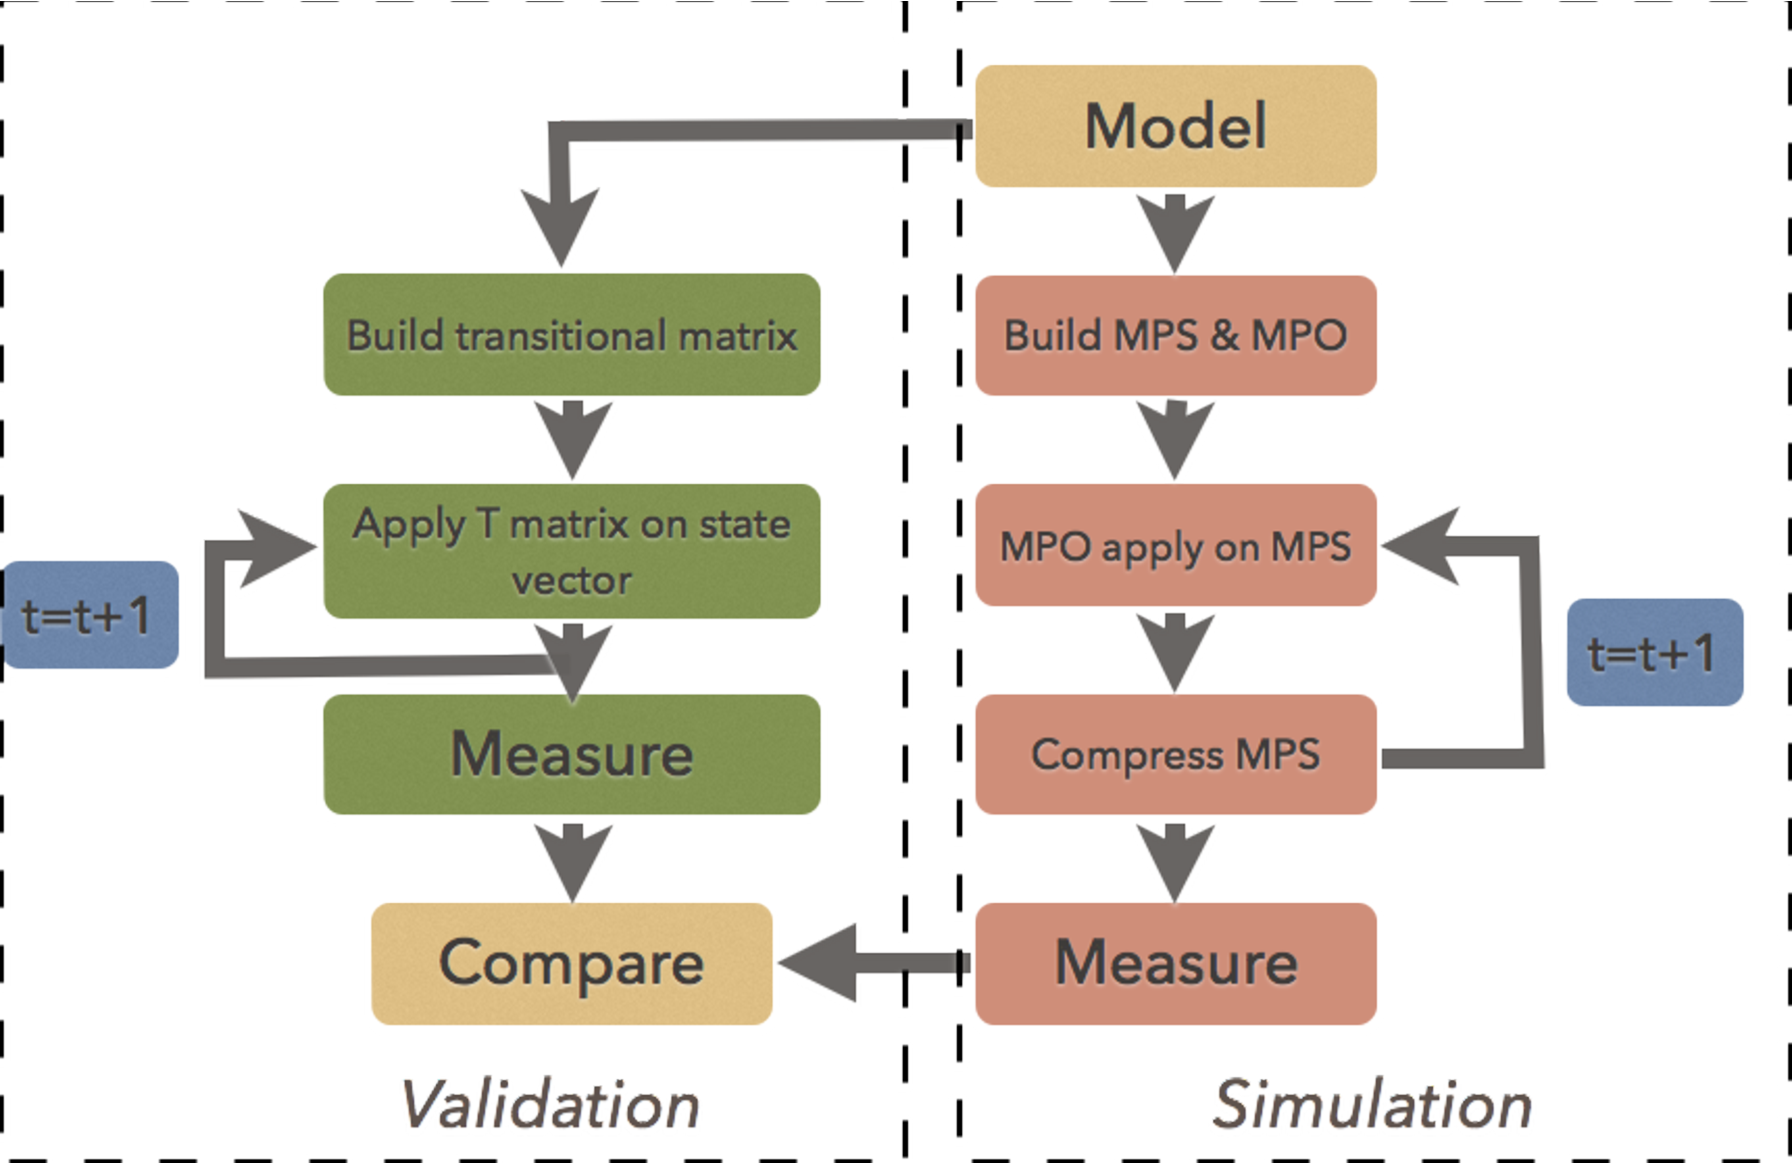
\includegraphics[width=0.7\textwidth]{flow_chart_new.pdf}
\caption{The flow chart of our program.}
\label{fig:flow_chart}
\end{center}
\end{figure}

\begin{figure}[htbp]
\begin{center}
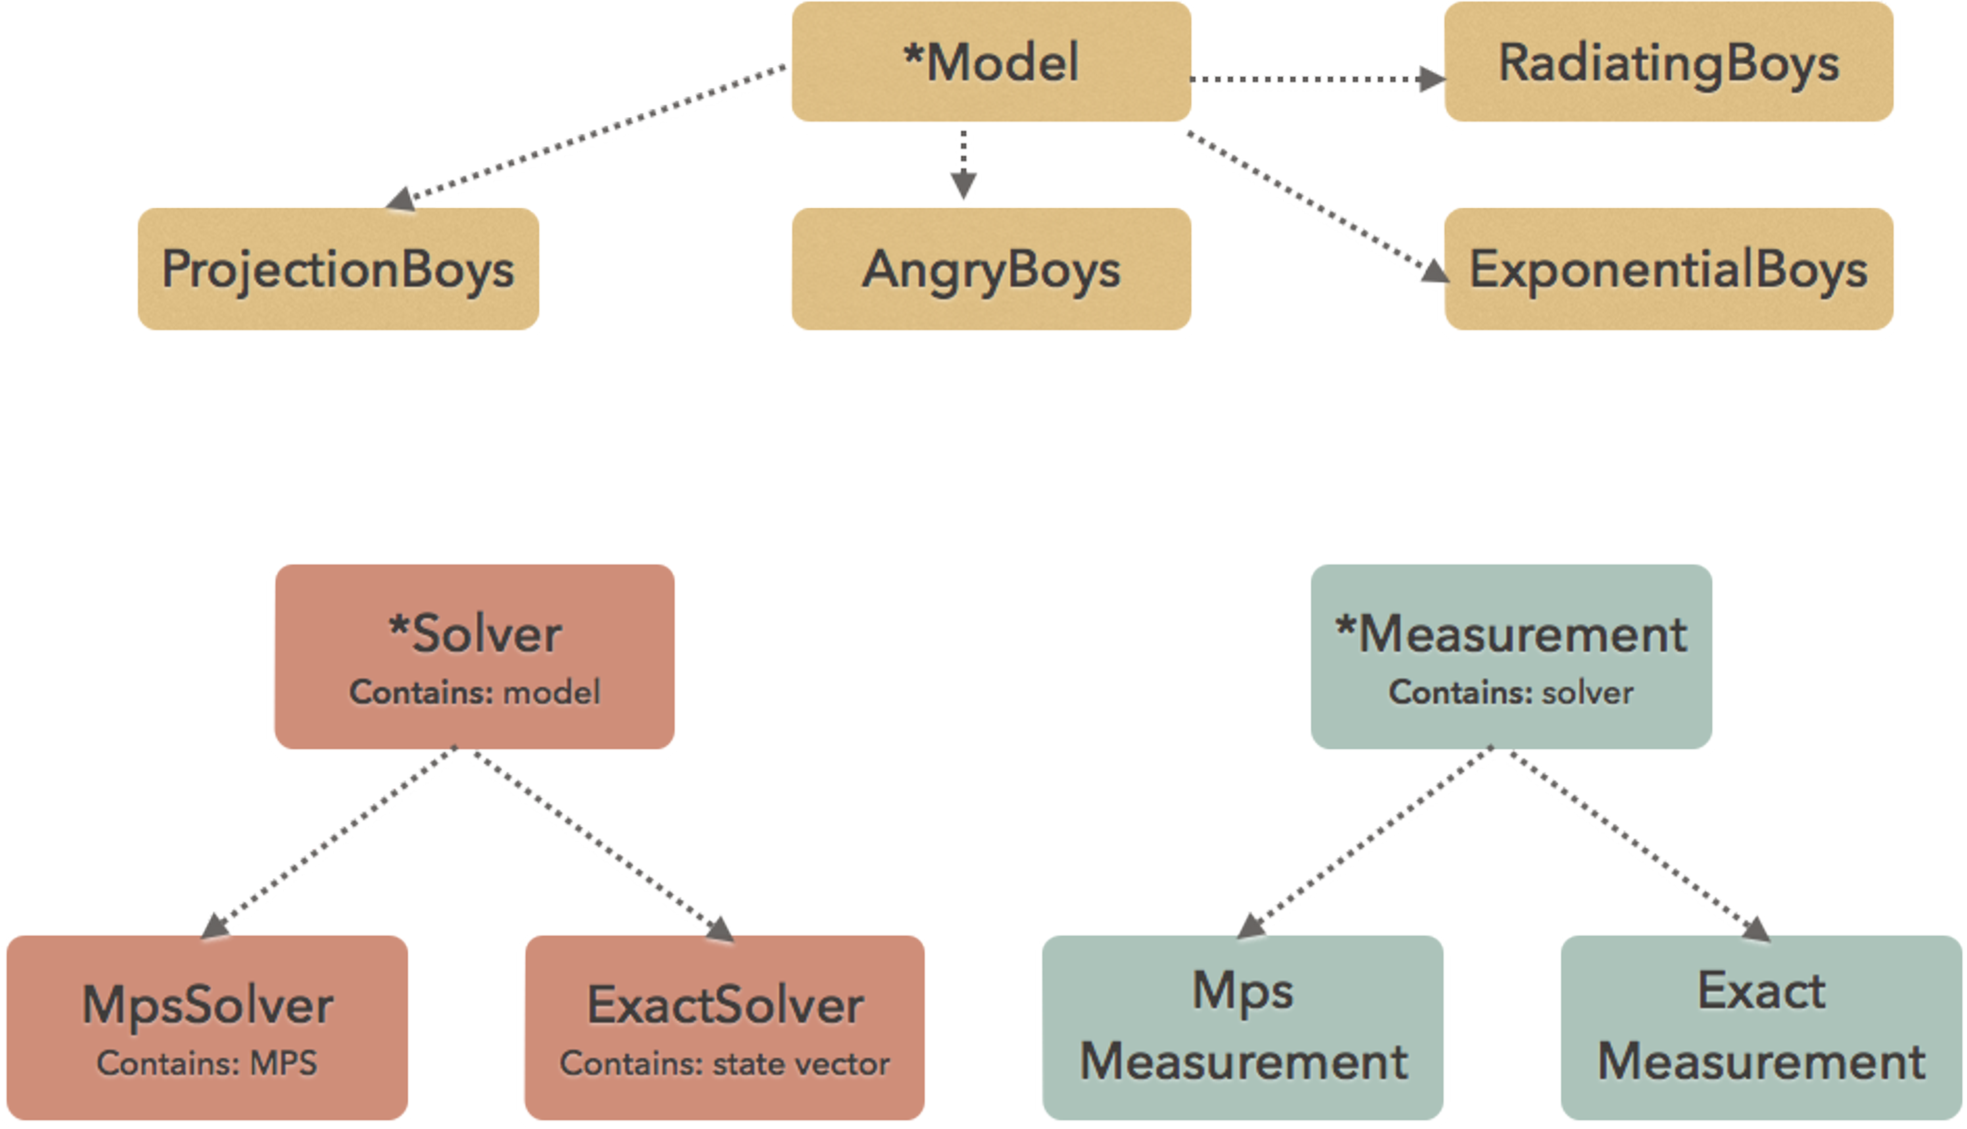
\includegraphics[width=0.7\textwidth]{class_diagram_new.pdf}
\caption{A bird view of our classes.}
\label{fig:class_diagram}
\end{center}
\end{figure}


The implementation is summarized in Fig.~\ref{fig:flow_chart}. The model is implemented in multiple ways. The classes used are described in Fig.~\ref{fig:class_diagram}.
\subsection{\texttt{Model} Class}
We defined an abstract model class in model.py which contains several frequently used components in the MPO. Each specific model is a derived class from Model class and they contain a string description of the model, model parameters, and a callable method to build the MPO/MPS representation and the transitional matrix for the user.
\subsection{\texttt{ExactSolver} Class}

\subsubsection{Solving the Problem in Theory}
	The many body problem is treated one dimensionally, with $n$ agents on a line at positions $i=1,2,\cdots,n$. Each body can occupy one of two states $(1,0)^T$ and $(0,1)^T$, corresponding to a state space of size $2^n$. The dynamics of the system at each time step can be represented by the following probability transition matrix:
\begin{displaymath}
H = pI + (1-p)\sum_{i=1}^{n-1}\frac{1}{n-1}\sigma_i^x\otimes\sigma_{i+1}^x,
\end{displaymath}
where $I$ is a $2^n\times2^n$ identity matrix and
\begin{displaymath}
\sigma_i^x =
\begin{pmatrix}
0 & 1 \\
1 & 0
\end{pmatrix}
\end{displaymath}
operates on the state space of position $i$.  Qualitatively, the transition matrix models the system by capturing interactions between neighboring bodies. A body's state remains constant with probability $p$, and flips its state with probability  $(1-p)/(N-1)$. Consider the $Angry Boys$ model as an example: the system is an abstraction of boys standing in a line, and their mood is in a state of either  "anger" $(1,0)^T$ or "tranquility" $(0,1)^T$. Their respective states are in turn influenced by their left and right neighbors.

\subsubsection{Solving the Problem Computationally}
	Simulating a solution to the many body problem is computationally intense. Construction of the transition matrix at each time step requires a summation over $N$ indices of $\sigma_{i}$
simultaneously, meaning $m^{N}$ terms are examined. For a simply model where a body occupies one of two elemetary states, $m^{N}\approx10^{9}$ for $N=30$. A simulation of $40$ sites is impossible.  Nonetheless, an exact solution class \texttt{ExactSolver} bounded by reasonably-sized state spaces has been constructed as a corroboration of results obtained through the MPS algorithm.

The \texttt{ExactSolver} class takes the \texttt{Solver} class as its parent. Its dependencies include the \texttt{numpy} library, the deepcopy function of the \texttt{copy} library, and a \texttt{Boys} model from its respective parent class. Three functions defined in the class - \texttt{interpreter}, \texttt{step}, and \texttt{evolve} - conduct simulation. Data from the simulation is collected in the form of lists. One list saves the state of the model at each time step, and one list saves the sum of probabilities at each step to ensure proper normalization of the model (probability cannot exceed 1).

The \texttt{interpreter} function accepts the imported model, reads its information, and initiates the simulation. The model's information consists of the beginning transition matrix and the initial state. Once the transition matrix is set, and the initial state is set and saved, simulation can commence. This represents a change from the alpha version; orginally, \texttt{interpreter} itself was used to initiate the transition matrix and initial state. The beta version now offers functions to do this so that models with more diverse properties can interact with the solver. For instance, models reflecting influence from only a left or right neighbor can direct their unique transition matrix to \texttt{ExactSolver}. Additional control over initial state conditions is also given.

The \texttt{step} function is very simple. It first increments simulation time, and then produces a new state by calculating the tensor dot product of the transition matrix and previous state.

The \texttt{evolve} function controls the flow of the simulation by taking as its argument the total number of time steps desired for the simulation. \texttt{evolve} calls \texttt{step} to produce a new state, and then appends this state and its norm to its respective data list. This process is done iteratively for the number of time steps, producing a time evolution of the model. 


\subsection{\texttt{MpsSolver} Class}
Parallel to the class \texttt{ExactSolver}, we construct a class named \texttt{MpsSolver} to store the MPS representation of the current state, to hold the MPO representation of the dynamics of the system and to comprise several functions necessary to updating the current state. 
\subsubsection{Member variables}
We have the current state saved under a variable named \texttt{mps}, which is a 3-d array storing $M^{\sigma_i}_{a_{i-1},a_i}$. The operator $O^{\sigma_i, \sigma'_i}_{n_{i-1}, n_i}$ is stored in a variable named \texttt{mpo}, which is a 4-d array. After applying the MPO on the MPS, we do the compression and the result is stored in \texttt{mpsc}. In addition, we store the time of the system in the variable \texttt{t}. These are variables defining the current state of the system. In addition, \texttt{MpsSolver} also hosts parameters and auxiliary variables used by overlap, compression and other routines in the class. For example, \texttt{bound\_dimension} defines the dimension of the compressed MPS.
\subsubsection{Methods}
The key method in the \texttt{MpsSolver} class is \texttt{step()} which updates the system from $t$ to $t+1$. The updating process involves three steps: (i) applying MPO on MPS (ii) compressing MPS to the desired size. (iii) normalizing the compressed state. We implement \texttt{contraction} to realize step 1, which simply involves some basic operations of multiplication of arrays and summing over a certain number of indices. For the compression step, we implement two methods: \texttt{compressionSVD}, and \texttt{compressionVariational} from which the user can choose which to use. \texttt{normalizeProba} is implemented to normalize the compressed MPS so that it becomes a probability distribution. Finally, we also implement \texttt{evolve()} to allow the user to update the system a certain number of times.
\subsubsection{Compression by variation}
The main routine for compression by variation is \texttt{compressionVariational}. It does the following operations:
\begin{itemize}
\item \texttt{initializeMpscVar}: Form a initial guess of the compressed MPS of desired size. It is then left or right canonized, depending on the direction of the first sweep. $L^2-$distance with the original MPS is calculated. 
\item \texttt{initializePartialOvl}: Initialize the partial overlap lists. Note that if the first sweep is from left to right, then we only have to initialize the right partial overlaps.
\item \texttt{compressionSweepLeftRight}: Perform a sweep from left to right. For each site, we calculate the matrix using left and right partial overlap. Before moving to the next site on the right, we have to left-normalize the current site (to preserve the mixed-canonical form) and update the left partial overlap list. At the end of the sweep, we calculate the $L^2-$distance with the original MPS and store the value in \texttt{cpr\textunderscore err}.
\item \texttt{compressionSweepRightLeft}: Perform a sweep from right to left. The idea is the same as described above.
\item We start the sweep with direction specified by the user and alternate the left and right sweeps until the $L^2-$distance recorded by \texttt{cpr\textunderscore err} converges.
\end{itemize}
Throughout the sweeps, we also keep track of the $L^1-$norm of the MPS. The User can choose whether to normalize the MPS after each sweep or after the completin of all sweeps.




\subsection{\texttt{Measurement} Class}
The \texttt{Measurement} class includes functions for calculating joint probability, correlations among multiple sites and mean as well as variance for a particular site at any time point. For the last two calculations, user can define specific values for being angry (up) or calm (down), and by default, they are 1 and -1 respectively. Both time and site number counts from 0, and a python-way of specifying the number from the end of list is also accepted. Each measurement task must specified in the particular way, though measurement time can be omitted, in which case it is taken to be the most recent time computed. Note in each task tuple, the integer following the task name will always be taken as the time step for all measurement. For more details, please consult the user manual or the sample program.



\subsubsection{\texttt{ExactMeasurement} Class}

The measurement in exact calculations is straightforward. Since each site has only 2 distinct states, any definite state of the system can be encoded as a binary number, i.e., in  the program, the down state is encoded as 0 and up state is encoded as 1, and the random state of the system at any time is fully specified by giving the probability of all definite states. From these full joint (in terms of each site) distributions, all quantities at a particular time point can be computed from marginalization. Moreover, the average value of given site is a special case of general correlation function, which is an average of a sequence of sites, and from the average value the variance of a given site can be easily computed by using appropriate up and down values.



\subsubsection{\texttt{MpsMeasurement} Class}

The measurement in the MPS case is a little bit more complicated since we are not directly specifying full joint probability distributions as in the exact calculation. However, from the definition of MPS, we can see that for a particular definite state of the system which is encoded as $s_0s_1\cdots s_{L-1}$, where $s_i=0$ or $1$ for any $i$ and $L$ is the length of the chain, its probability can be computed from a matrix product 
\begin{displaymath}
P(s_1s_2\dots s_{L-1}) = M_0^{s_0}M_1^{s_1}\cdots M_{L-1}^{s_{L-1}}
\end{displaymath} 
where $M_i^{s_i}$ is the matrix representation of site $i$ being in the state $s_i$. Since the matrices at first and last site are row and column vectors respectively, in the end we will obtain a number as expected. From these full joint probability distributions, we then can obtain all measurement quantities at a particular time as in the exact calculation. There is also a little trick to speed up the marginalization by using the distributive law in matrix multiplication. For example, if we want to compute the joint distribution of sites $i_1$, $i_2,\cdots,i_n$ in states $s_1$, $s_2,\cdots,s_n$, where, for simplicity, assuming $0<i_1<i_2<\cdots<i_n<L-1$, we then have the desired probability to be
\begin{displaymath}
P(s_{i_1}s_{i_2}\dots s_{i_n}) = (M_0^{0} + M_0^{1})\cdots M_{i_1}^{s_{i_1}}\cdots M_{i_2}^{s_{i_2}} \cdots M_{i_n}^{s_{i_n}} \cdots (M_{L-1}^{0} + M_{L-1}^{1})
\end{displaymath}
i.e, we add up the matrices representing up and down for all sites except sites $i_1$, $i_2,\cdots,i_n$, for which a particular matrix is chosen, and then multiply all matrices. Similarly, for a correlation as $\langle S_{i_1} S_{i_2} \cdots S_{i_n} \rangle$, where $S_i$ is the random variable representing the two possible states at site $i$, we can obtain it from
\begin{displaymath}
\langle S_{i_1} S_{i_2} \cdots S_{i_n} \rangle = (\sigma_0^0 M_0^0 + \sigma_0^1M_0^1)(\sigma_1^0M_1^0 + \sigma_1^1M_1^1)\cdots (\sigma_{L-1}^0M_{L-1}^0 + \sigma_{L-1}^1M^1_{L-1})
\end{displaymath}
where $\sigma_i^0=\sigma_i^1=1$ for all sites except $i_1$, $i_2,\cdots,i_n$, where $\sigma_i^0=$ specified value for down state and $\sigma_i^1=$ specified value for up state. 
\vspace{3mm}

\section{Results}
\subsection{AngryBoys Model}
    Fig.\ref{fig:Angry_result} describes the main data that we obtained through the MPS method. The Angryboys Model was used. Fig.\ref{fig:Angry_result}a is the comparison between the compressed MPS method and the exact MPS method when the chain size $L=10$ and the bound dimension $\chi=10$. We calculated time evolution of the joint probability, the mean value, and the variance to find that the compressed MPS method agrees well with the exact method. Furthermore, in this model, all three quantities reach a limit at large enough time, indicating that this model is an aperiodic Markov chain. In Fig.\ref{fig:Angry_result}a, we examined the square error sum of the joint probability between the compressed MPS method and exact method at different bound dimension $\chi$. The figure clearly shows that the error decreases almost exponentially with the increasing bound dimension; and when the bound dimension is close or above 10, the error can be neglected for short chains. This confirms that our approximation is valid. Fig.\ref{fig:Angry_result}c gives the result for a long chain, where $L=100$ and $\chi=10$. Such a long chain case cannot be computed by the exact method since the size of the matrix grows exponentially with chain length. However with our compressed method, we can calculate the physical properties of this long chain in a short time. Here we only use a small bound dimension $\chi=10$ and the size of the matrix is not very large. Thus the MPS method has greatly reduced the computation load in this problem. And the result also reaches an equilibrium state. Fig.\ref{fig:Angry_result}d compares the time evolution of the joint probability of MPS method when the bound dimension $\chi$ is 10 and 20 respectively. At early time, the two bound dimensions will generate slightly different physical quantities, but in the long run, the two cases will converge. Such a converging behavior shows that a bound dimension around 10 can already provide a good approximation of a long chain in Angryboys Model. It indicates that our compressed matrices can simulate the exact result well in the long run, although the matrices have been truncated a great deal. However, we must admit that when the chain size grows larger than 200, the code has some errors and interruptions.
    
\begin{figure}[H]
\centering
\subfigure[Exact Model(Short Chain)]{
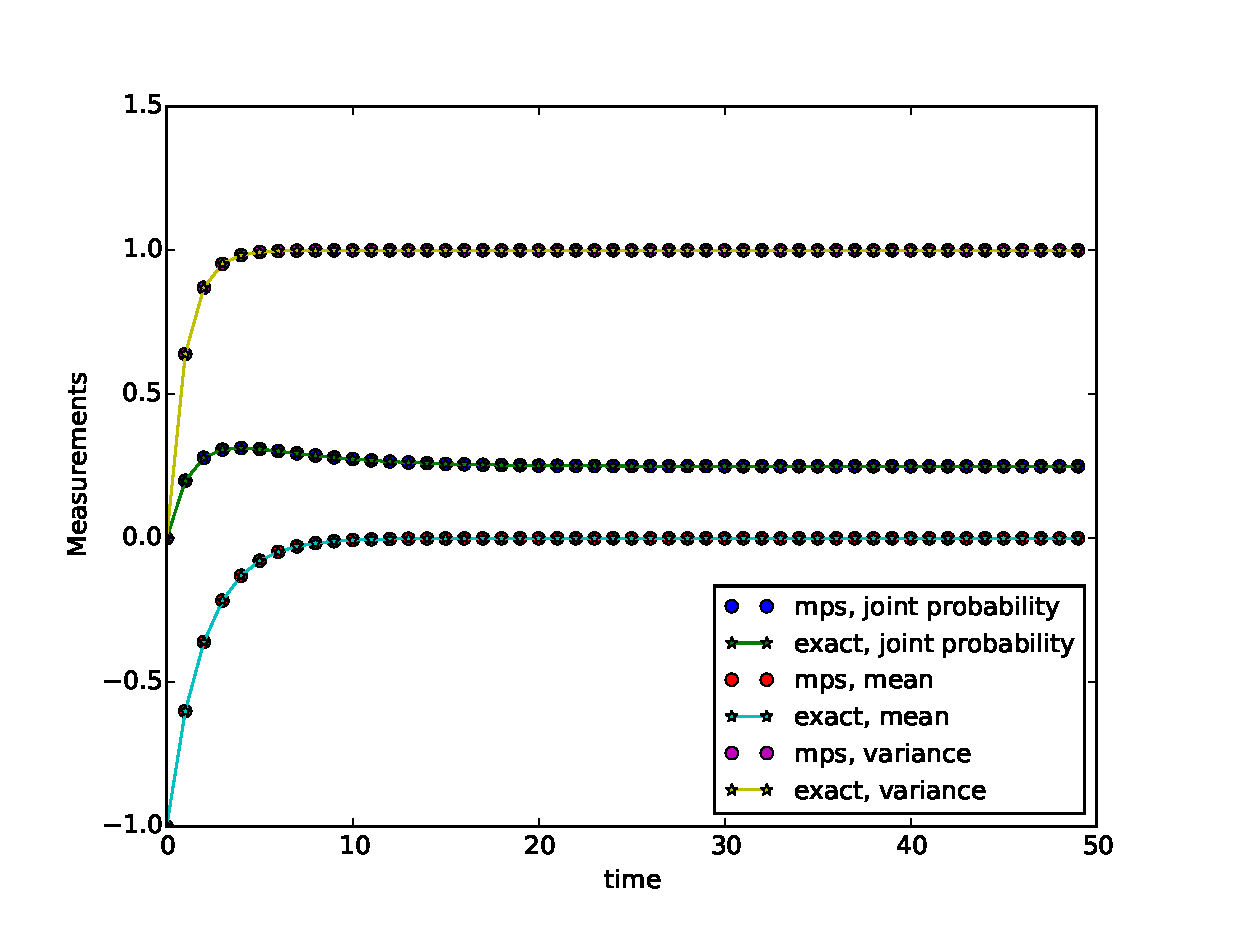
\includegraphics[scale=0.4]{Result_Fig/Angry_Exact_t50_s10_bd10.eps}}\hfill
\subfigure[Error with Different Bound Dimension]{
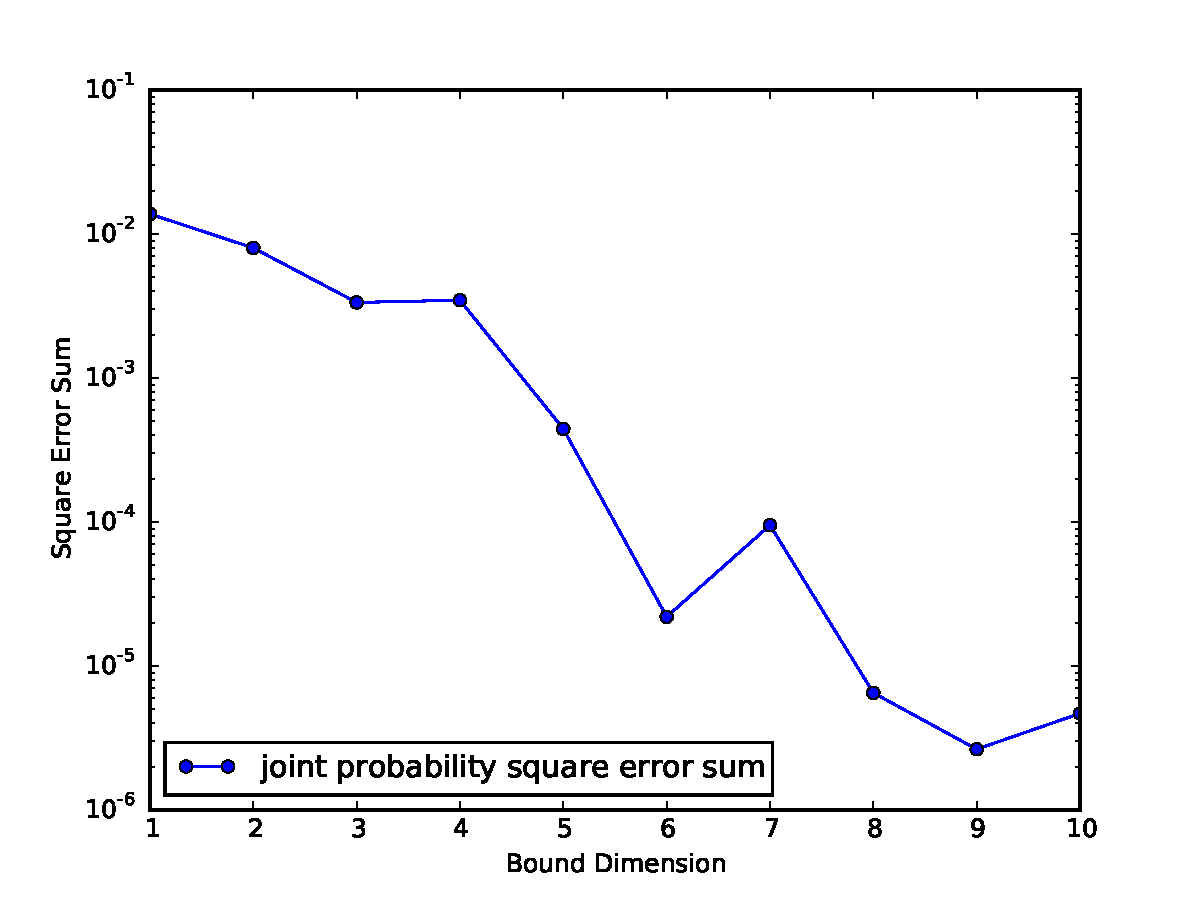
\includegraphics[scale=0.4]{Result_Fig/Angry_Error_t100_s10_bd10_log.pdf}}
\subfigure[MPS long chain]{
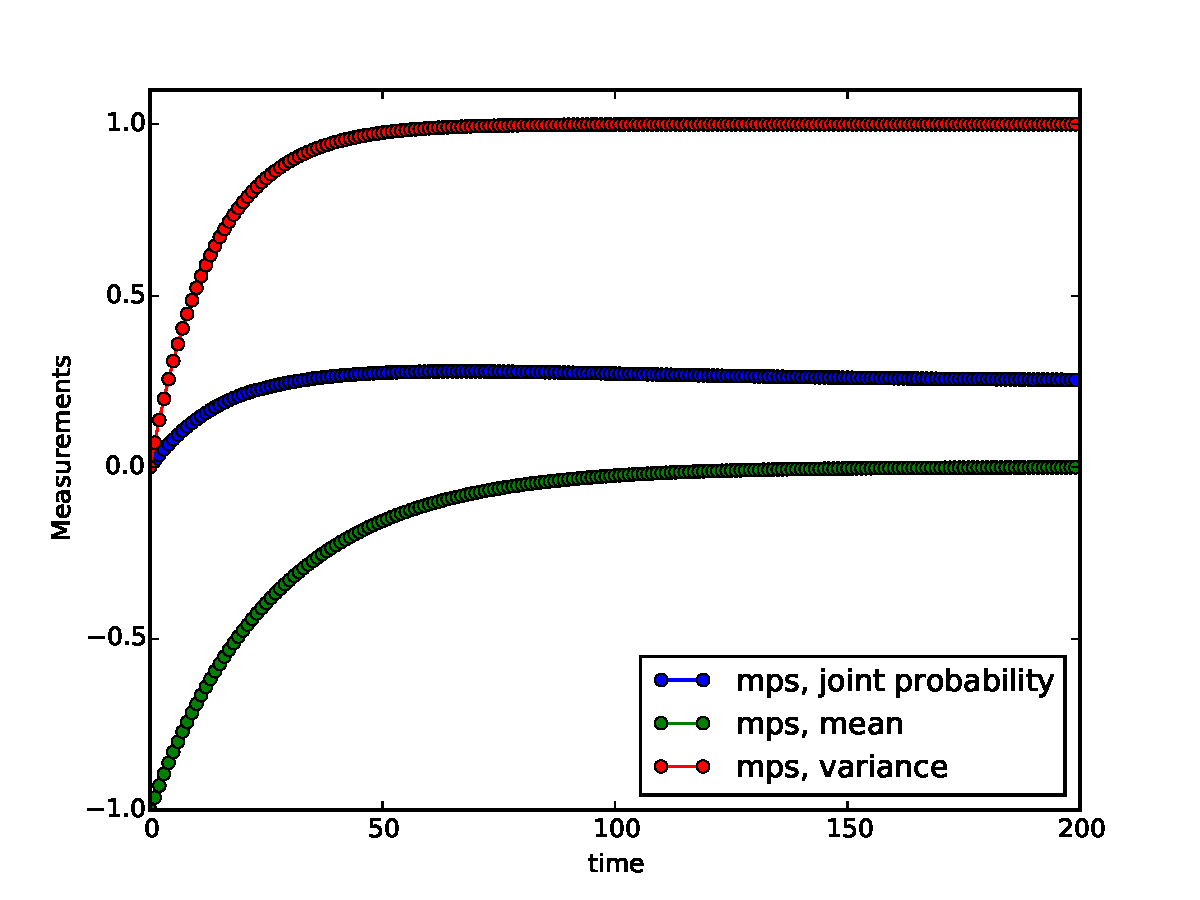
\includegraphics[scale=0.4]{Result_Fig/Angry_MPS_t200_s100_bd10.pdf}}\hfill
\subfigure[MPS with Different Bound Dimension]{
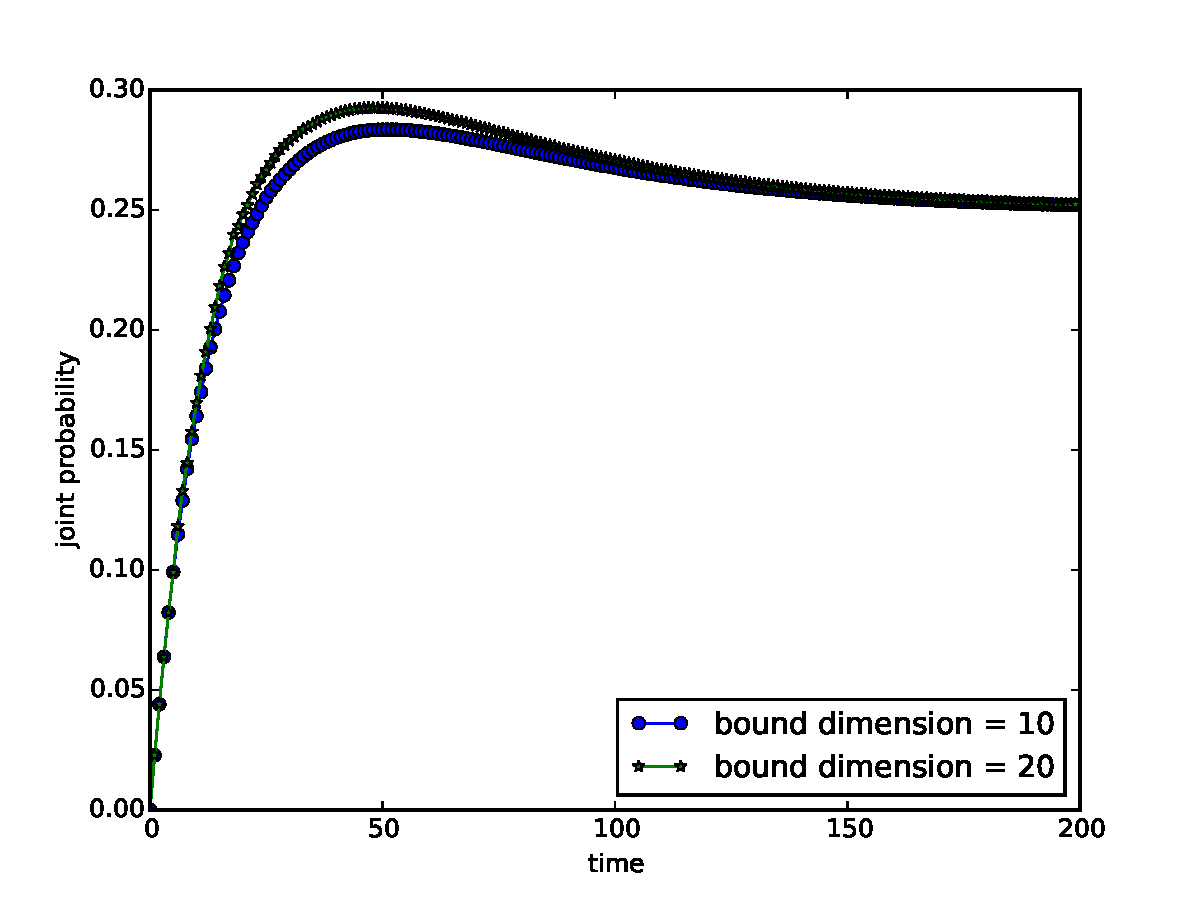
\includegraphics[scale=0.4]{Result_Fig/Angry_MPS_t200_s80_bd10to20.pdf}}
  % \end{minipage}\\[1em]
  \caption{Results of Angry Boys Model.(a) gives the comparison of the joint probability, the mean value, and the variance between the MPS method and exact method. The chain size is 10, and the bound dimension $\chi$ is 10 in the MPS method. (b) shows the decay of square error sum with increasing bound dimensions. The error is computed between the approximation and exact method with a fixed time step of 100. (c) is the result of MPS method on a long chain with the size $L=100$. (d) compares the joint probability of the MPS method with two bound dimensions. The two curves converge in the long run.}
  \label{fig:Angry_result}
\end{figure}

\subsection{RadiatingBoys Model}
Fig.\ref{fig:Radiating_result} is the result of the Radiating Boys Model. 
\begin{figure}[H]
\centering
\subfigure[Exact Model(Short Chain)]{
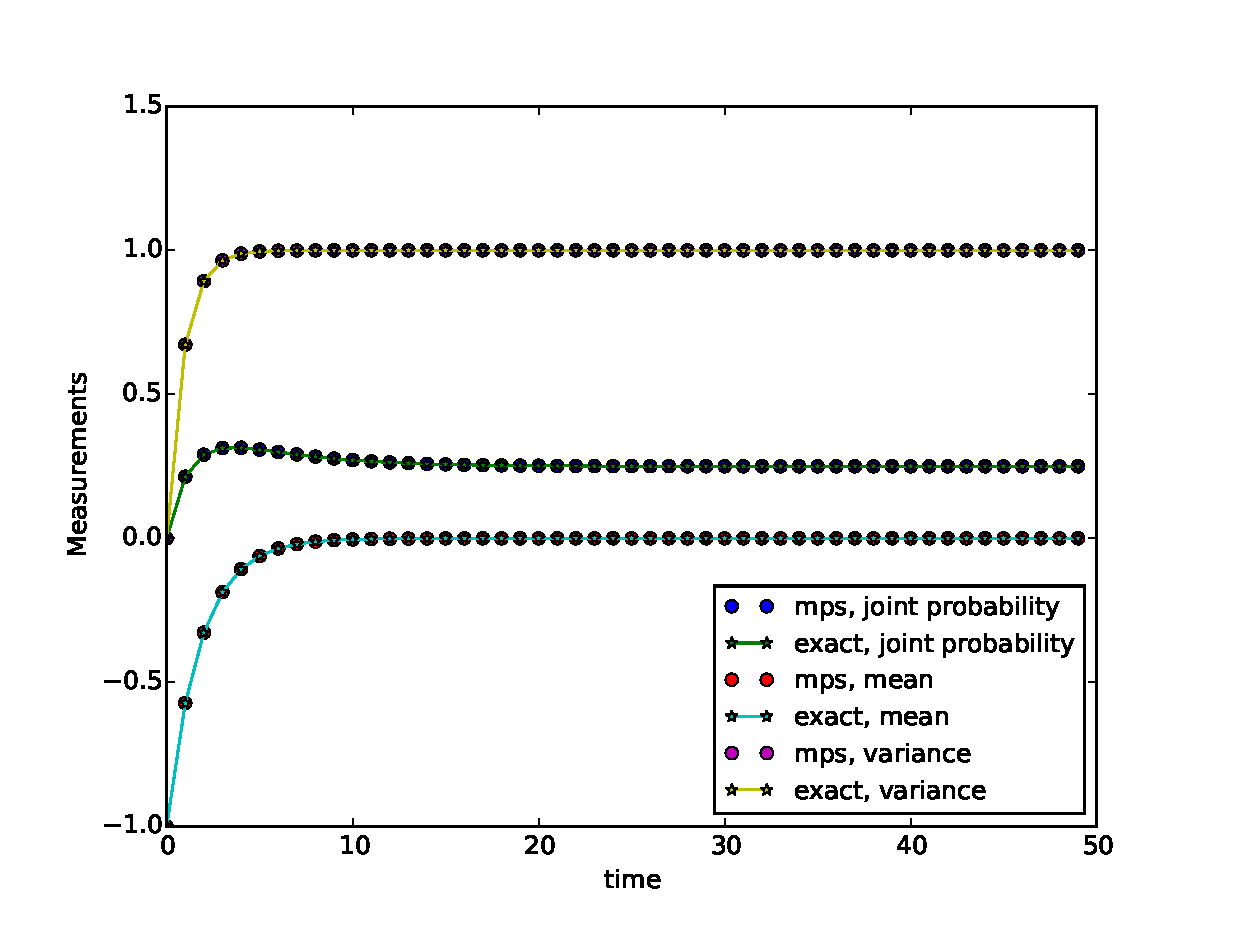
\includegraphics[scale=0.4]{Result_Fig/Radiating_Exact_t50_s10_bd10.eps}}\hfill
\subfigure[Error with Different Bound Dimension]{
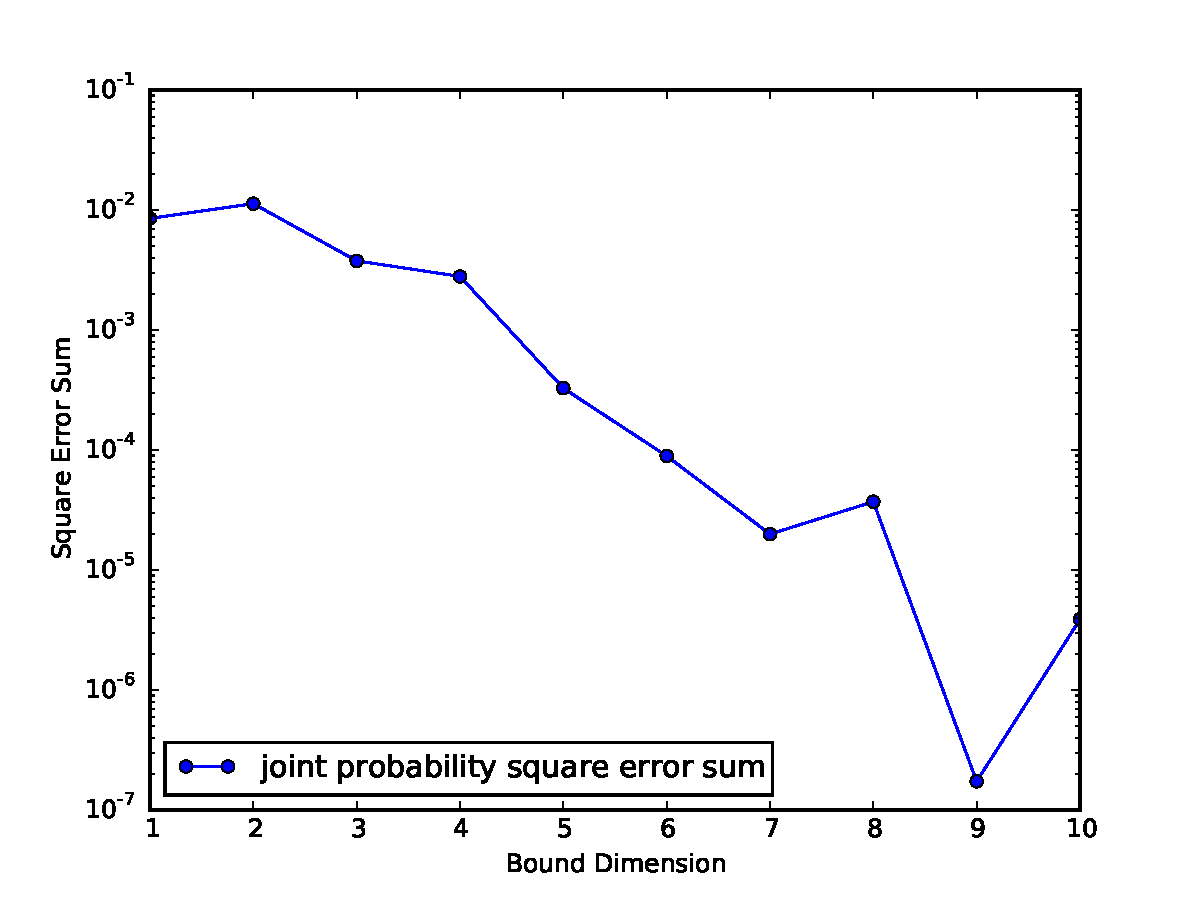
\includegraphics[scale=0.4]{Result_Fig/Radiating_Error_t100_s10_bd10_log.pdf}}
\subfigure[MPS long chain]{
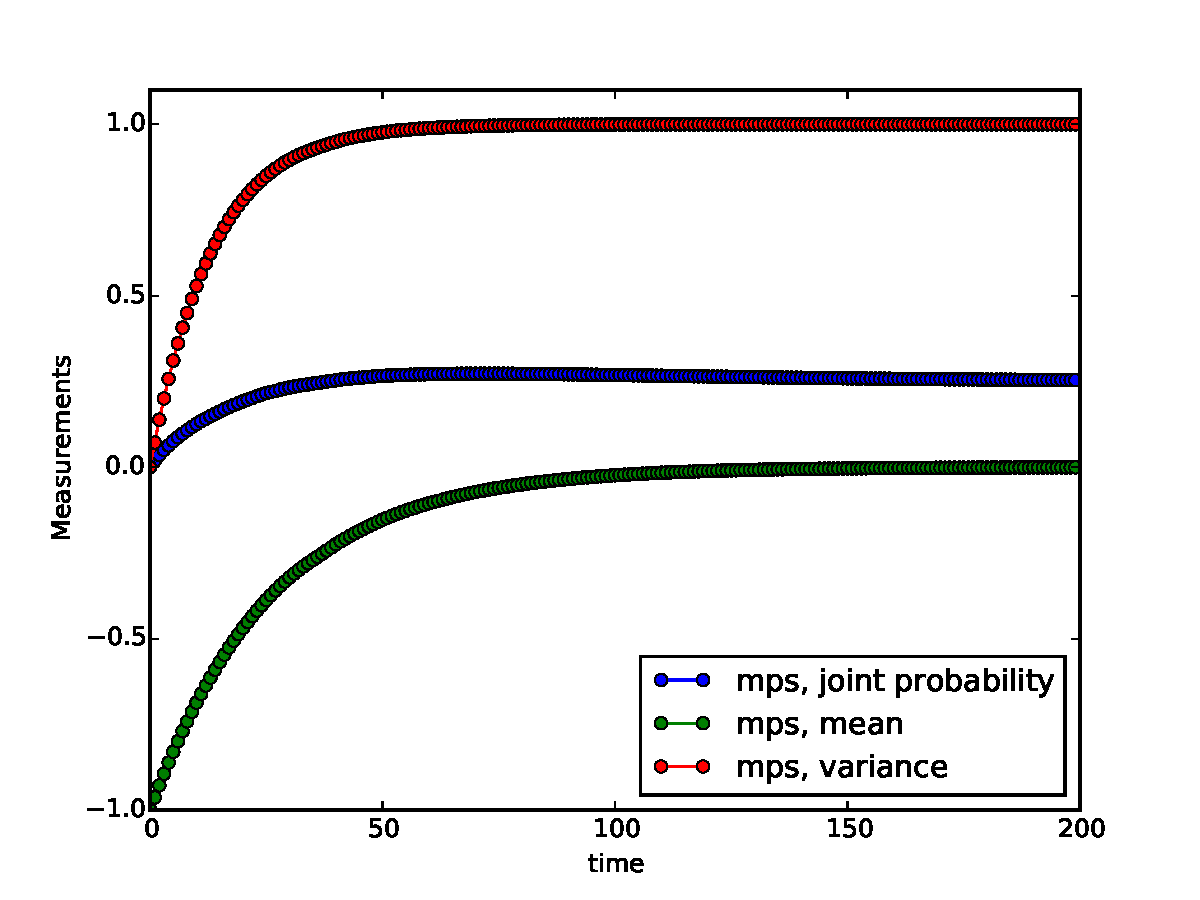
\includegraphics[scale=0.4]{Result_Fig/Radiating_MPS_t200_s100_bd10.pdf}}\hfill
\subfigure[MPS with Different Bound Dimension]{
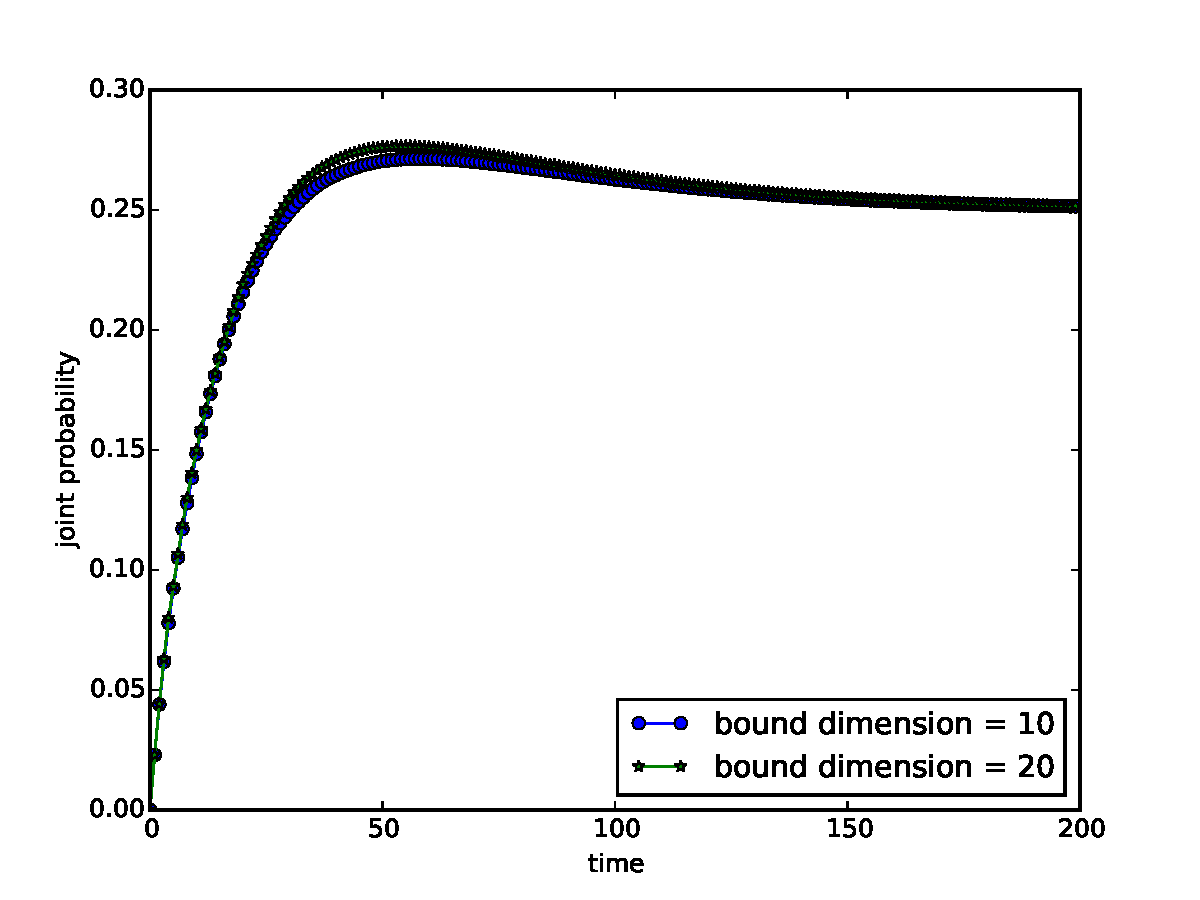
\includegraphics[scale=0.4]{Result_Fig/Radiating_MPS_t200_s80_bd10to20.pdf}}
  % \end{minipage}\\[1em]
  \caption{Results of Radiating Boys Model.(a) gives the comparison of the joint probability, the mean value, and the variance between the MPS method and exact method. The chain size is 10, and the bound dimension $\chi$ is 10 in the MPS method. (b) shows the decay of square error sum with increasing bound dimensions. The error is computed between the approximation and exact methods with a fixed time step of 100. (c) is the result of the MPS method on a longer chain with size $L=30$. (d) compares the joint probability of the MPS method with two bound dimensions. The two curves converge in the long run.}
  \label{fig:Radiating_result}
\end{figure}

\subsection{ExponentialBoys Model}
Fig.\ref{fig:Exponential_result} is the result of the Exponential Boys Model. 
\begin{figure}[H]
\centering
\subfigure[Exact Model(Short Chain)]{
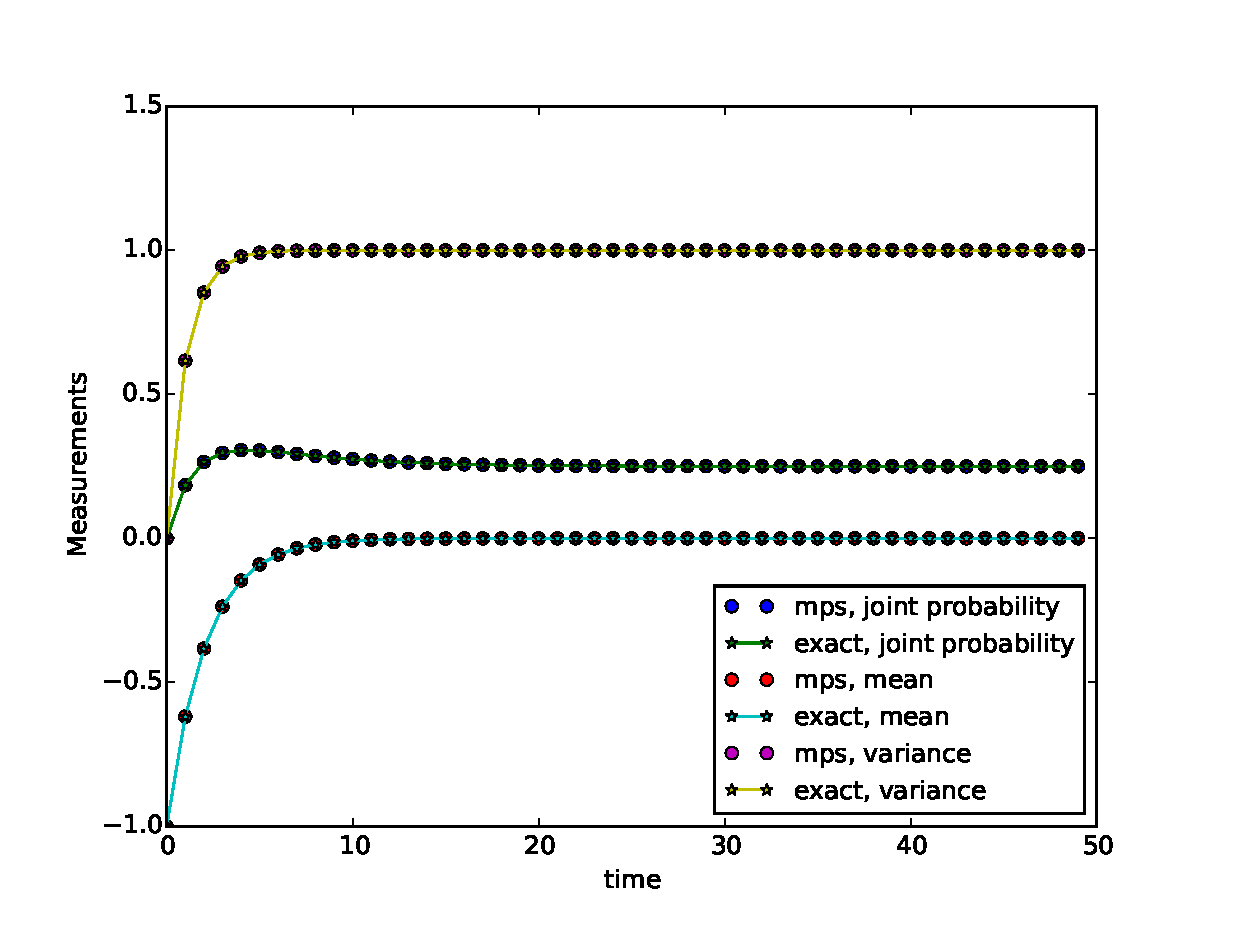
\includegraphics[scale=0.4]{Result_Fig/Exponential_Exact_t50_s10_bd10.eps}}\hfill
\subfigure[Error with Different Bound Dimension]{
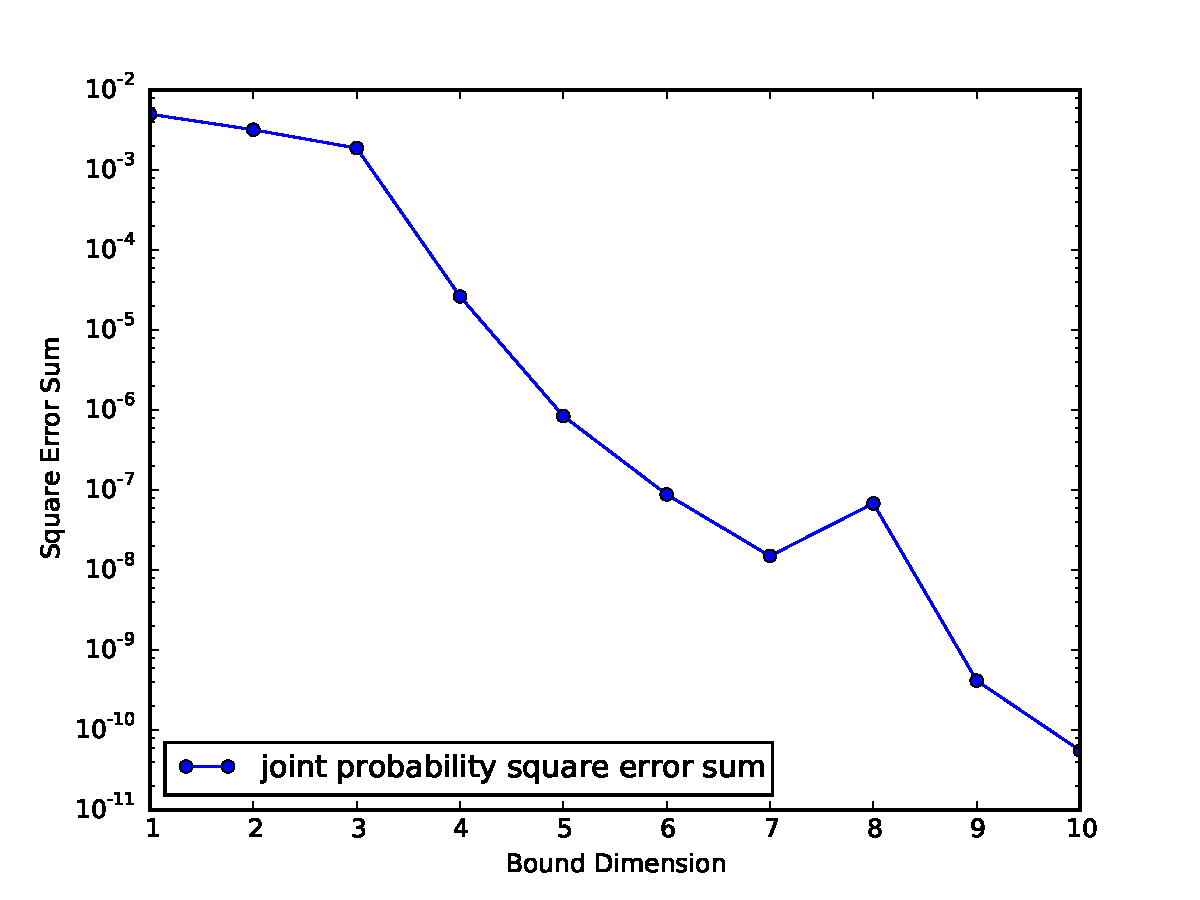
\includegraphics[scale=0.4]{Result_Fig/Exponential_Error_t100_s10_bd10_log.pdf}}
\subfigure[MPS long chain]{
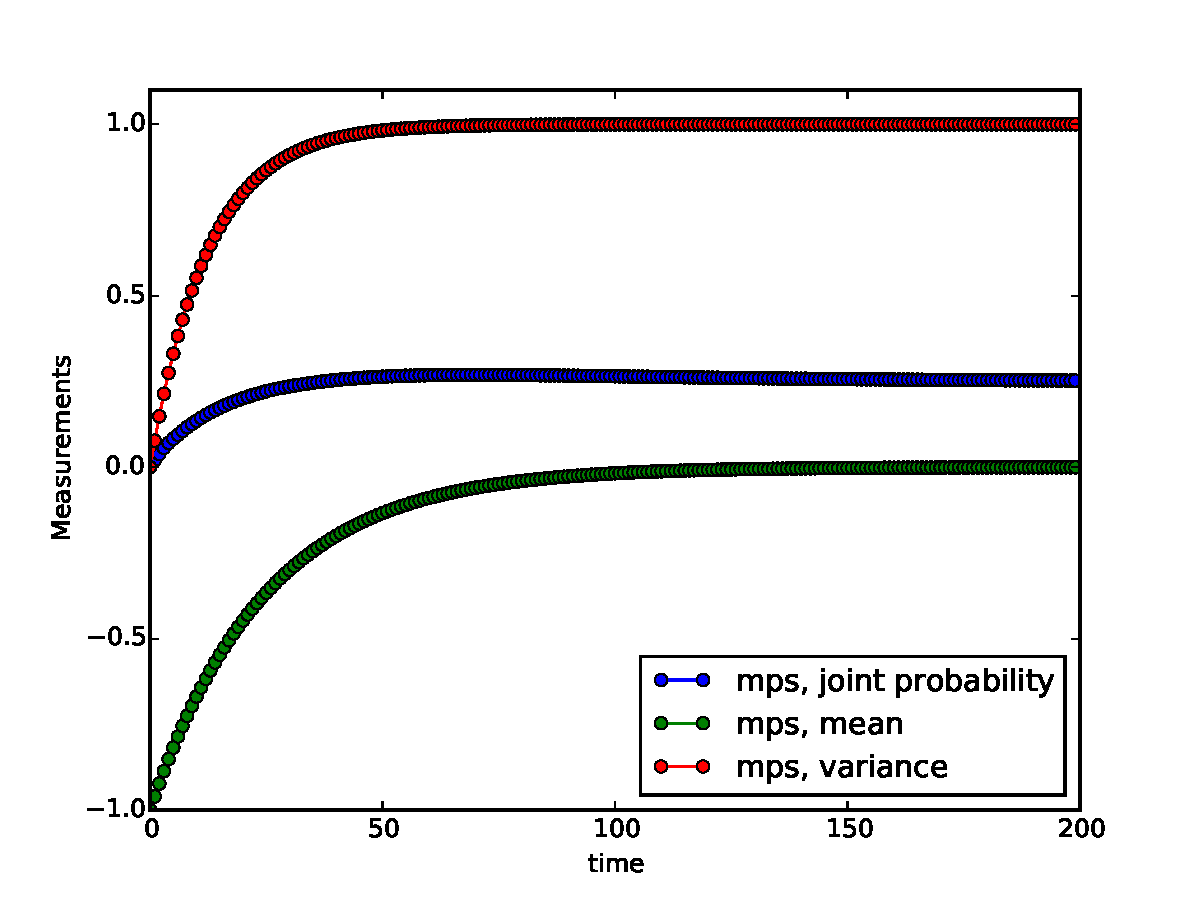
\includegraphics[scale=0.4]{Result_Fig/Exponential_MPS_t200_s100_bd10.pdf}}\hfill
\subfigure[MPS with Different Bound Dimension]{
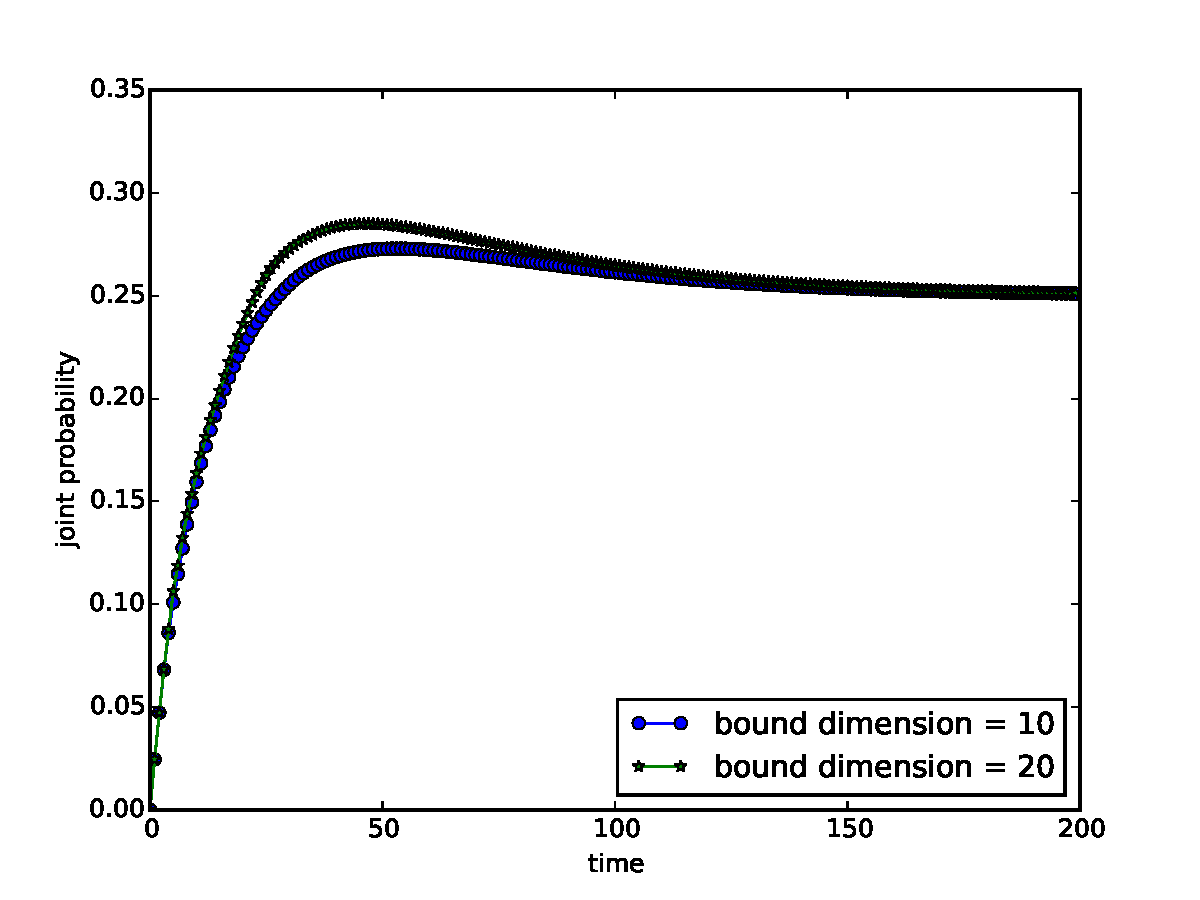
\includegraphics[scale=0.4]{Result_Fig/Exponential_MPS_t200_s80_bd10to20.pdf}}
  % \end{minipage}\\[1em]
  \caption{Results of Exponential Boys Model.(a) gives the comparison of the joint probability, the mean value, and the variance between the MPS method and exact method. The chain size is 10, and the bound dimension $\chi$ is 10 in the MPS method. (b) shows the decay of square error sum with increasing bound dimensions. The error is computed between the approximation and exact methods with a fixed time step of 100. (c) is the result of the MPS method on a longer chain with the size $L=40$. (d) compares the joint probability of the MPS method with two bound dimensions. The two curves converge in the long run.}
  \label{fig:Exponential_result}
\end{figure}

\subsection{ProjectionBoys Model}
Fig.\ref{fig:Projection_result} is the result of the Projection Boys Model.
\begin{figure}[H]
\centering
\subfigure[Exact Model(Short Chain)]{
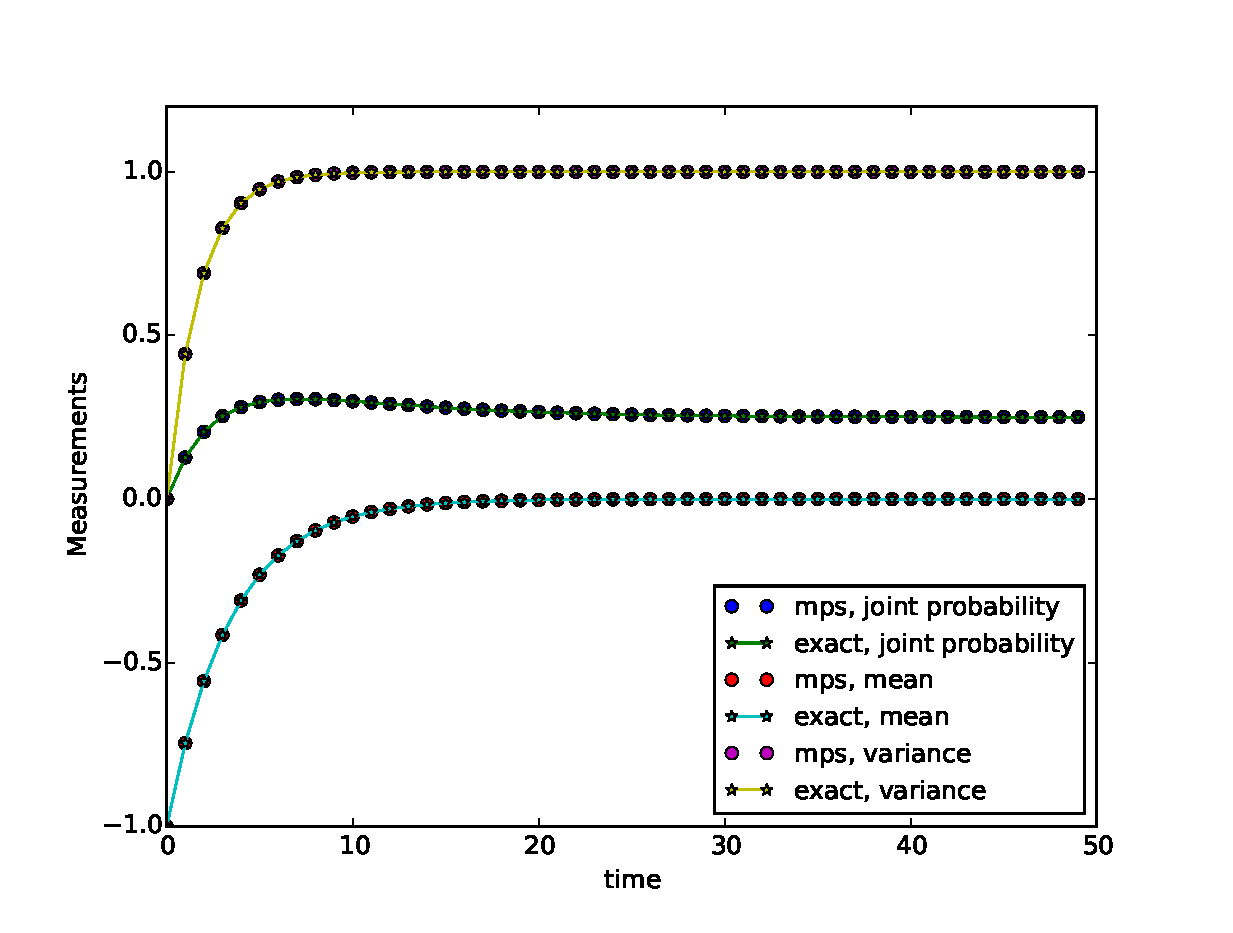
\includegraphics[scale=0.4]{Result_Fig/Projection_Exact_t50_s10_bd10.eps}}\hfill
\subfigure[Error with Different Bound Dimension]{
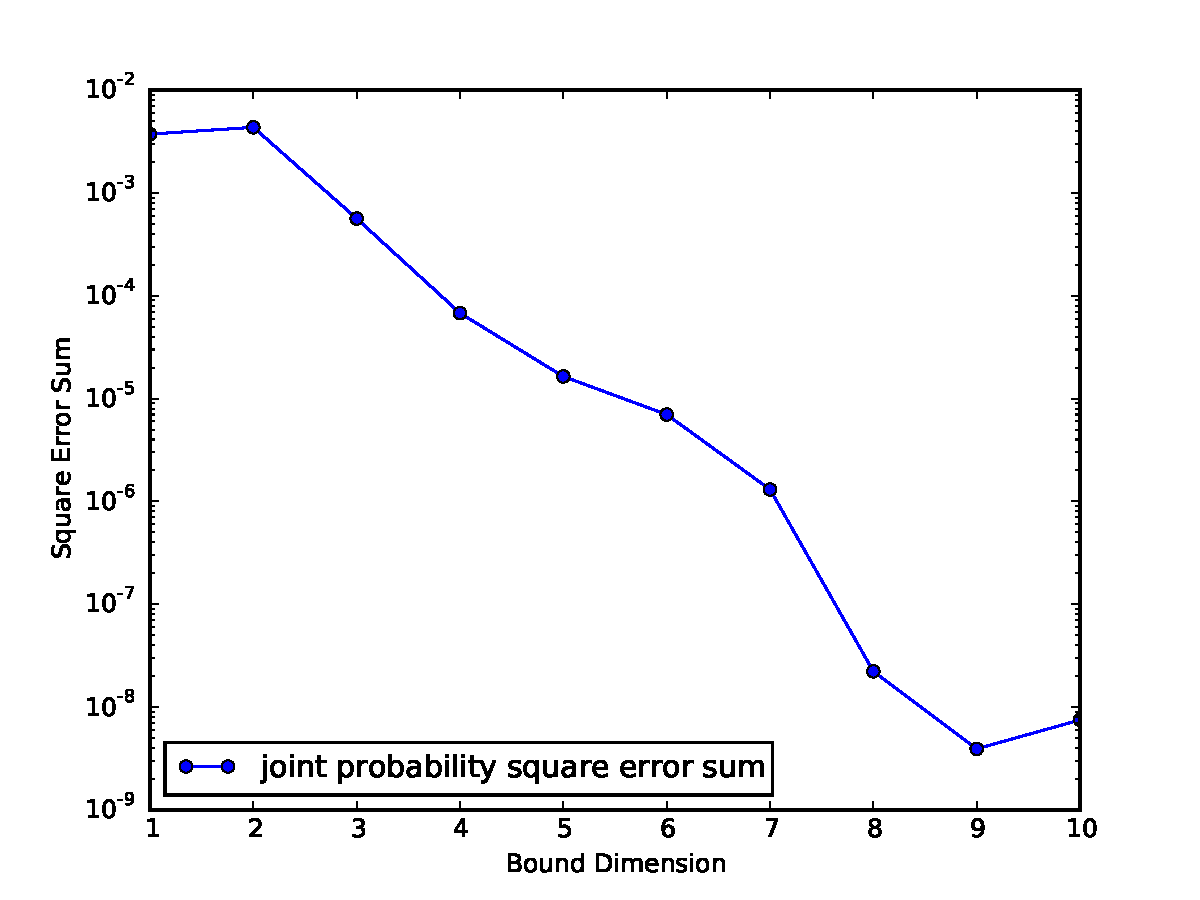
\includegraphics[scale=0.4]{Result_Fig/Projection_Error_t100_s10_bd10_log.pdf}}
\subfigure[MPS long chain]{
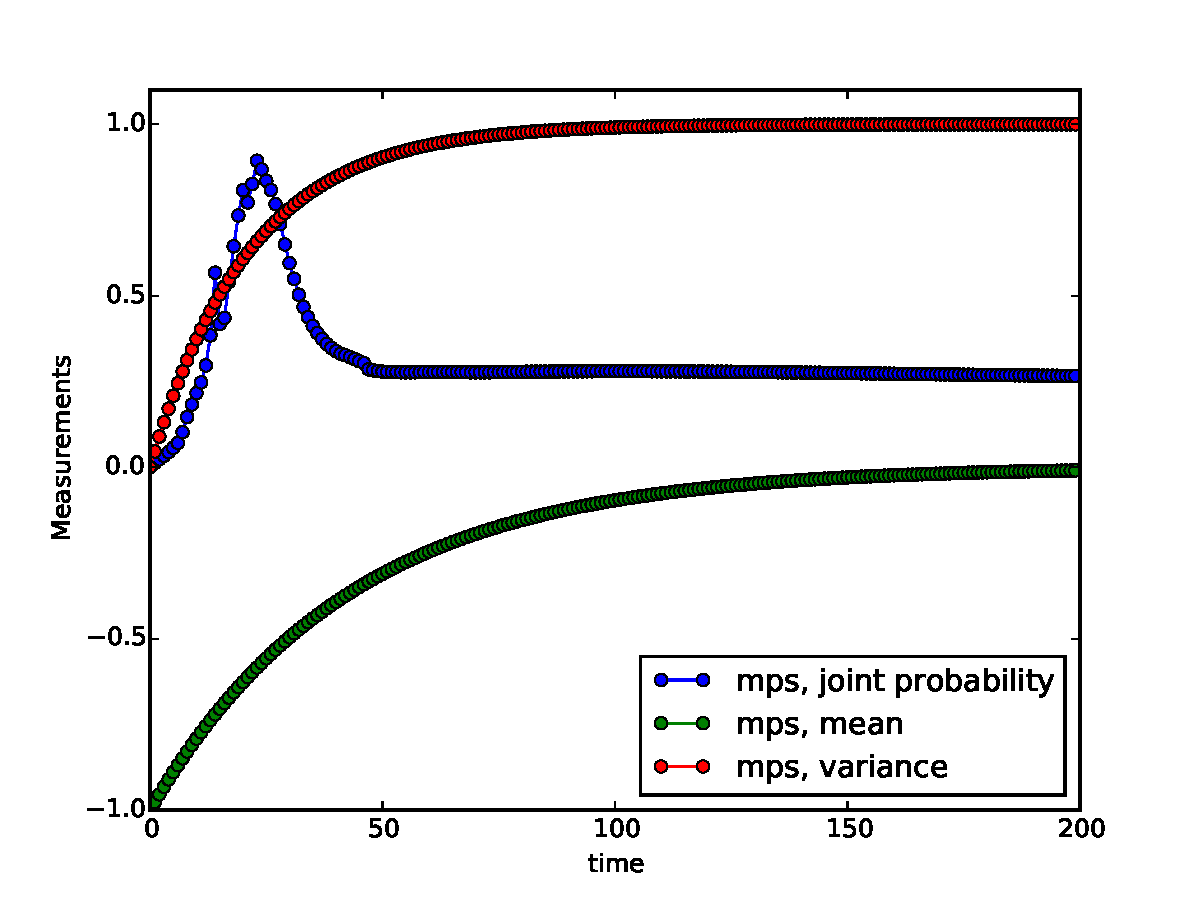
\includegraphics[scale=0.4]{Result_Fig/Projection_MPS_t200_s100_bd10.pdf}}\hfill
\subfigure[MPS with Different Bound Dimension]{
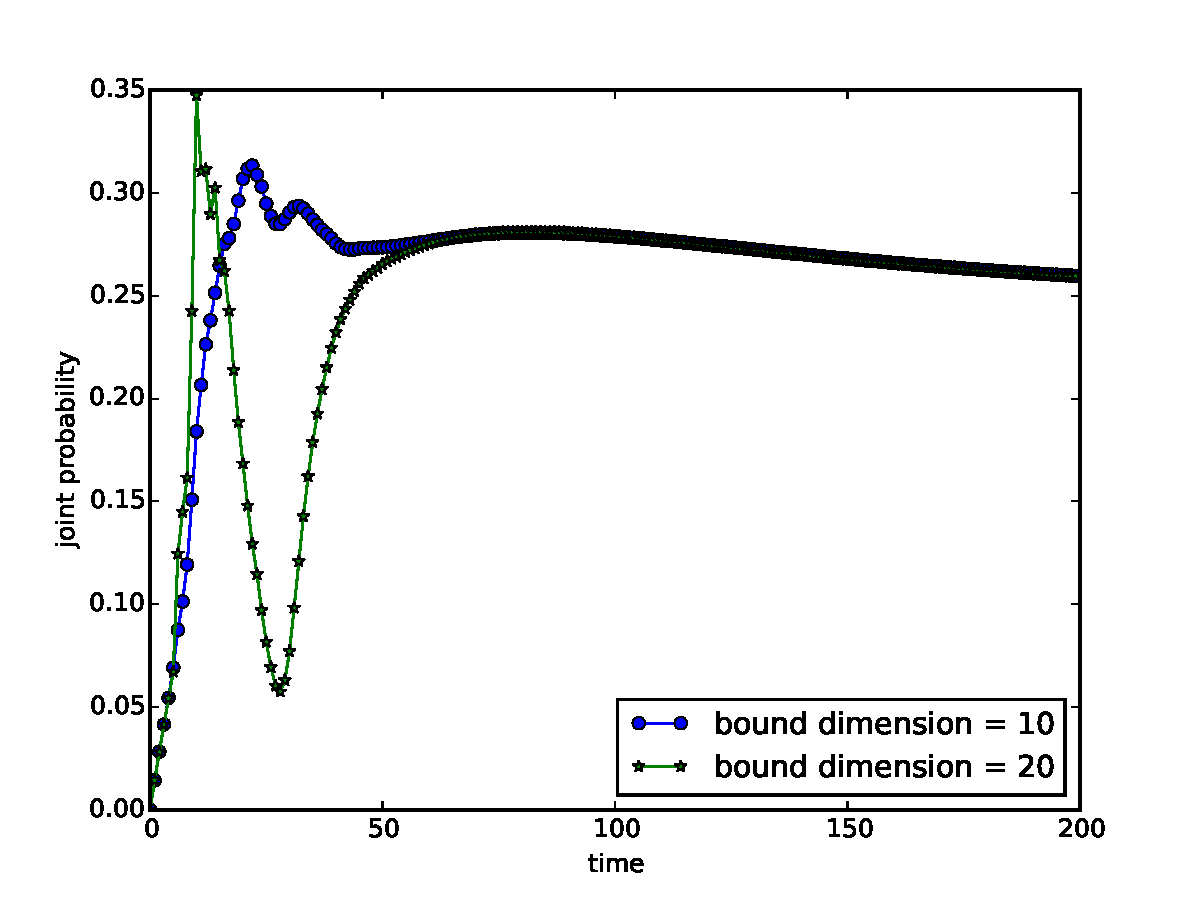
\includegraphics[scale=0.4]{Result_Fig/Projection_MPS_t200_s80_bd10to20.pdf}}
  % \end{minipage}\\[1em]
  \caption{Results of Exponential Boys Model.(a) gives the comparison of the joint probability, the mean value, and the variance between the MPS method and exact method. The chain size is 10, and the bound dimension $\chi$ is 10 in the MPS method. (b) shows the decay of square error sum with  increasing bound dimensions. The error is computed between the approximation and exact methods with a fixed time step of 100. (c) is the result of the MPS method on a long chain with the size $L=150$. (d) compares the joint probability of the MPS method with two bound dimensions. The two curves converge in the long run.}
  \label{fig:Projection_result}
\end{figure}

\section{Profiling}
To have an idea of how time is consumed in our MPS solver, we pick an angry model boy of length 100 and make it evole for $t=5$. We pick $10$ the bound dimension for compression. Fig.\ref{fig:prof} shows the output of calling cProfile. It takes 40.049 seconds in total to finish the computation. We observe that 33.197 seconds are consumed by the function \texttt{tensordot()}, which basically handles all the n-dimensional array multiplication. Indeed \texttt{tensordot()} comes with the \texttt{numpy} package which has already been implemented by some lower-level languange and optimized for intensive computation. Therefore we believe that implementing our project in C++ will not significantly accelerate the computation. 
\begin{figure}[H]
\centering
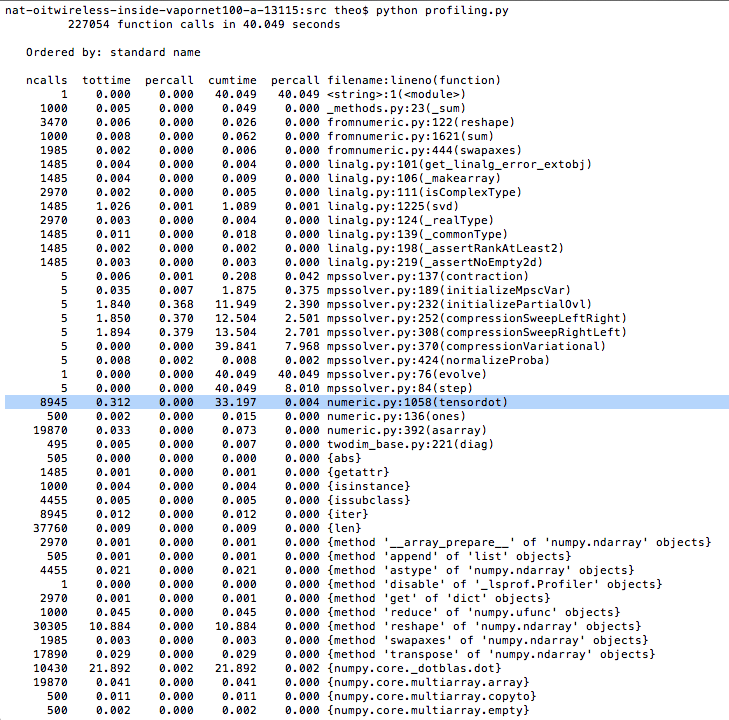
\includegraphics[scale=0.4]{Result_Fig/profiling.png}
\caption{Output of Cprofiling on executing \texttt{evolve(5)} for an angry boy model. The highlighting line shows the time consumed by the function \texttt{tensordot}}
\label{fig:prof}
\end{figure} 

\section{Conclusion}
From Newton's famous invention of calculus, to differential equations in the 19th century, fiber bundles in modern geometry, and tensor category in modern algebra inspired by particle physics; there can be no doubt physics research has stimulated many ideas in mathematics for centuries. We believe that, as physics has adopted computer technology over the past several decades, it should also inspire more ideas in computer science. This project is an attempt at attaining this goal.

The structures in quantum many body physicsgeatly  resembles classical probability theory, with the exception of interpreting the 2-norm rather than 1-norm as probability. Physicists developed many methods to compute the time evolution of states (or "wave functions") in the context of quantum mechanics, and we naturally extend this MPS approach to classical probability theory.

It is proved in the physics context that the bound dimension of the MPS does not grow with the chain length for a 1-D problem, which is called the area law. An intuitive way to understand is that, if the states in a finite range connect only to each other, a cut in the chain will break some "information sharing". Nonetheless, the amount of the broken information does not grow with the chain length. While it is unclear whether we have a similar "area law" in this probability context, it was well worth it to give it a try.

As our results have shown, the algorithm works very well for short and intermediate length chains, while we need a larger bound dimension to get a good result for the joint probability. The proper bound dimension is still an open question, but in most cases, a chain of length 200 can be solved with a bound dimension of 20.

\noindent \textbf{What did we learn?}

Developing code using group collaboration is not an easy process, but we managed it quite well. We held several design meetings in the beginning and discussed the algorithm quite thoroughly. The task assignment was very clear and everyone worked on different files to resolve any ensuing collisions easily. The process we could improve in the future is managin writing of the final report. We did not split sections in different files wisely, which caused many collision problems.
\newpage
\begin{thebibliography}{99}
\bibitem{white} S. R. White, {\it Physical Review Letters} {\bf 69}, 2863 (1992)
\bibitem{schollwock} Ulrich Schollwoeck, {\it Annals of Physics} {\bf 326}, 96 (2011)
\bibitem{cirac} Verstraete, F., and J. I. Cirac, (2004), arXiv:cond-mat/0407066v1
\bibitem{vidal}G. Evenbly, G. Vidal, {\it J Stat Phys} (2011) {\bf 145:} 891-918
\end{thebibliography}
\end{document}

